\chapter{Results and Discussion}\label{chap:resultsAndDiscussion}
For the test of the algorithm different scenarios have been chosen and simulations were conducted to test the efficiency and accuracy of the path planning. The scenarios chosen for the simulation describe common problems path planning algorithms need to be able to overcome in order to be usable for the navigation in unstructured environments.

The following scenarios were simulated and are analyzed in the following. While the scenarios are different with regard to obstacle configurations. The term Euclidean refers to the use of an unconstrained Euclidean distance heuristic; 2D A* refers to the unconstrained shortest distance heuristic, taking obstacles into account; Dubins refers to the constrained shortest Dubins curve heuristic, limited to one driving direction; and Reeds Shepp refers to the constrained shortest Reed Shepp curve heuristic allowing for two driving directions.

Dark grey areas are free space. Black areas are obstacles. Yellow paths represent the different configurations of the vehicle while traversing the path and are used to visually check paths for collisions. Pink arrows represent a forward motion of the vehicle, while purple arrows correspond to a reverse motion. If the path is not accompanied by either pink or purple arrows then the analytical expansion has directly connected the most promising current state and the goal state. Yellow dots represent the area the 2D A* search has visited. A gradient of colors represent the relative cost estimate of each cell among all cells of the 2D A* search.

%The first problem The problems are depicted in \Fref{fig:scenarioDeadEnd}, \Fref{fig:scenarioParkingStructure} and \Fref{fig:scenarioRandomObstacles}.

%\begin{figure}[h]
%    \includegraphicsTex{scenarioDeadEnd.pdf_tex}
%    \caption{The dead end scenario}
%    \label{fig:scenarioDeadEnd}
%\end{figure}
%
%\begin{figure}[h]
%    \includegraphicsTex{scenarioParkingStructure.pdf_tex}
%    \caption{The parking structure scenario}
%    \label{fig:scenarioParkingStructure}
%\end{figure}
%
%\begin{figure}[h]
%    \includegraphicsTex{scenarioRandomObstacles.pdf_tex}
%    \caption{The random obstacles scenario}
%    \label{fig:scenarioRandomObstacles}
%\end{figure}

\section{Simulation Results}

\subsection{Parking Structure}
The size of the binary obstacle grid for the parking structure scenario is 50\,m $\times$ 100\,m. The parking structure is horizontally divided by obstacles with two small passages connecting both sides. The passages have a width of 4 meters. In the scenario a path needs to be found from the initial state $x_s$ in the lower half, facing the top to a final state $x_g$ in the upper half facing the wall the bottom.

\subsubsection{Analysis}
\Fref{fig:scenarioParkingEuclidean} depicts the planners result using only a Euclidean heuristic. It can be seen that the planner finds a non colliding path that is close to the shortest possible path. The number of vertices the planner needed to expand for reaching the goal is 47559. The planner has searched the area around the start position with a bias towards the goal position. The solution path lies in the opposite direction of the search focus.

The found path in \Fref{fig:scenarioParking2D} is identical, however the 2D A* heuristic is used. The search progresses away from the goal biased towards the passage on the left. The number of vertices expanded is 4767.

\Fref{fig:scenarioParkingCost} shows the area explored by 2D A* and the colors represent the relative cost of each cell among all explored cells. Red areas are associated with the highest cost, blue areas with the lowest cost. When looking at the color gradient it can be seen that the found path follows the gradient very closely. Only at the beginning, when the vehicle is backing up the costs are increasing. 

\subsubsection{Discussion}
Since the Euclidean heuristic only accounts for relative distance between two points and has no information with regard to the obstacles in the environment it heavily underestimates the cost to the goal and drives the search in the wrong direction expanding almost one order of magnitude more vertices than the 2D A* heuristic, which gives a clear picture of the environment. Since the 2D A* heuristics is much more informed it underestimates the true cost much less, and hence avoids wasteful expansion of unpromising vertices. The found path in \Fref{fig:scenarioParking2D} follows the cost gradient in most parts, but since 2D A* does not account for the non-holonomic nature of the vehicle, it does not account for the vehicle's need to back up out of initial parking position.

\begin{figure}[h]
    \centering
    \begin{subfigure}[t]{\textwidth}
    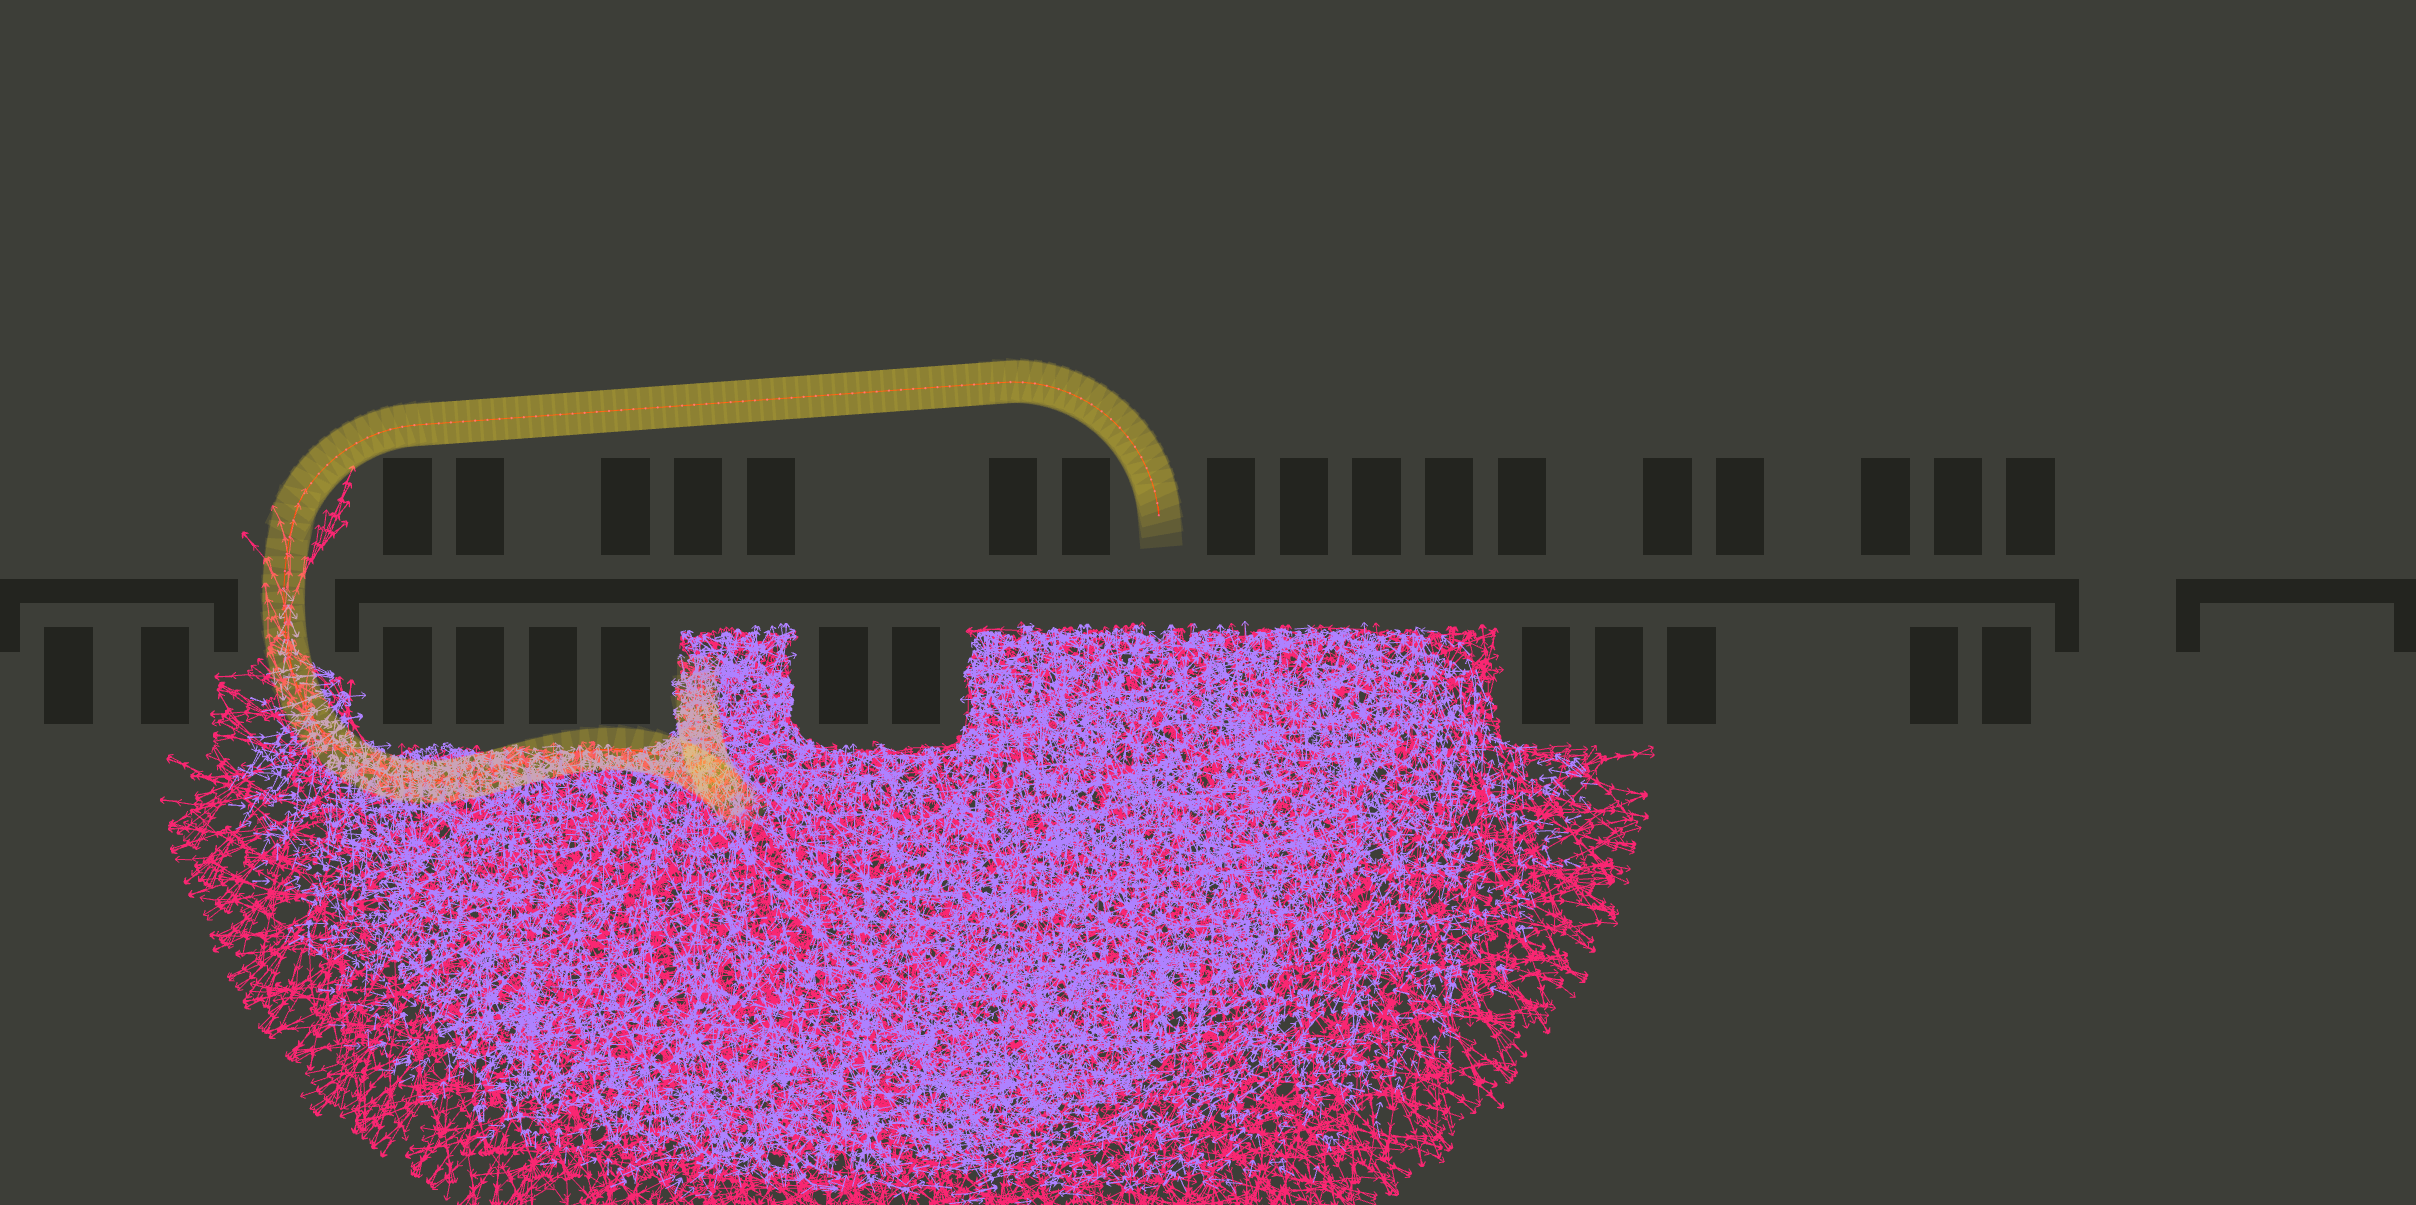
\includegraphics[width=\textwidth]{scenarioParking.png}
        \caption{Euclidean, 47559 vertices, length x\,m}
    \label{fig:scenarioParkingEuclidean}
    \end{subfigure}
    \begin{subfigure}[t]{\textwidth}
    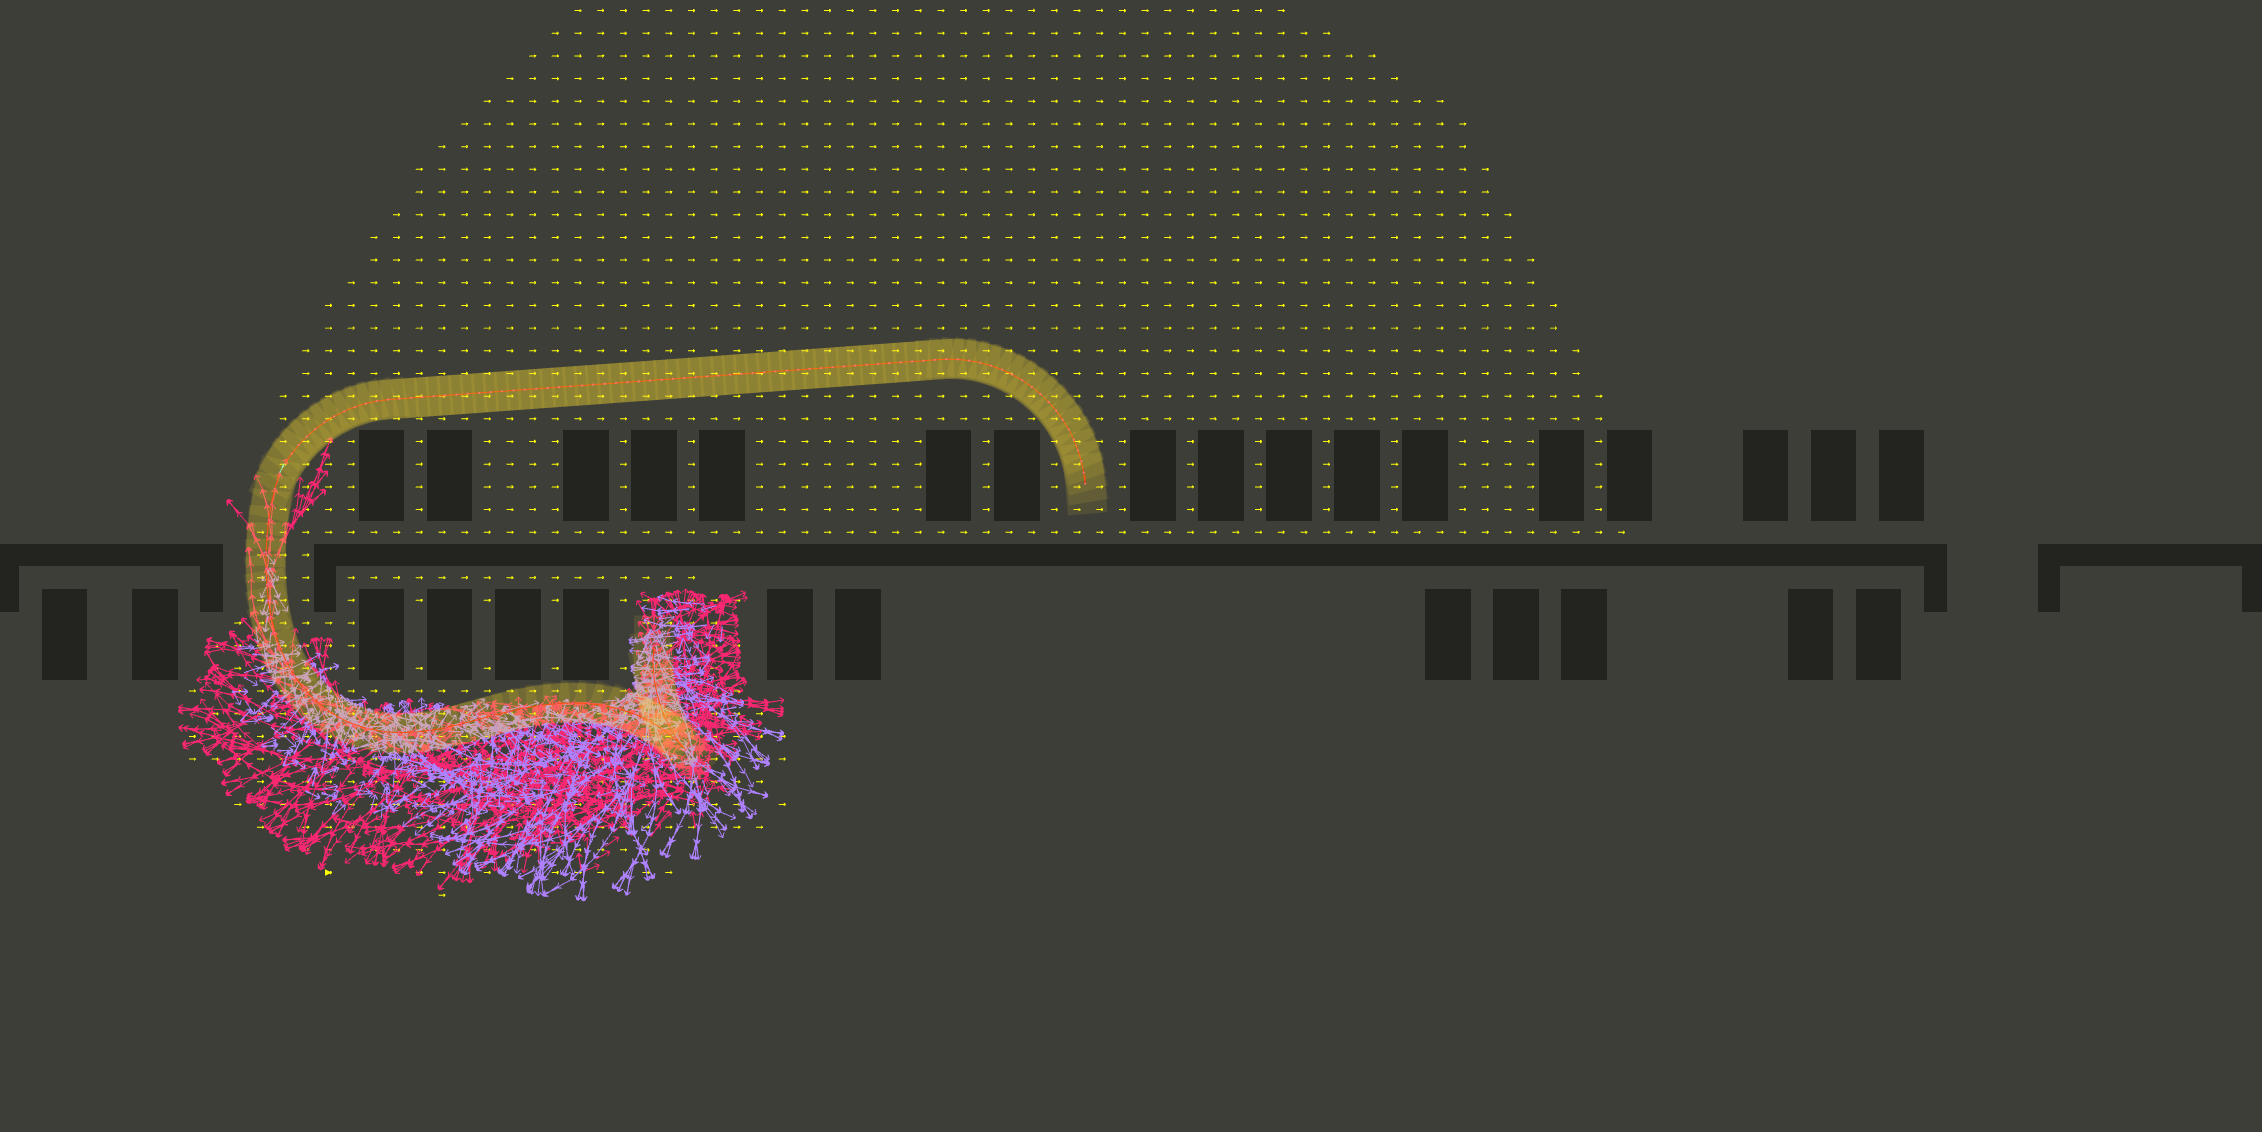
\includegraphics[width=\textwidth]{scenarioParking2d.png}
        \caption{2D A* \& Reeds Shepp, 4767 vertices (1517 vertices), length x\,m}
    \label{fig:scenarioParking2D}
    \end{subfigure}    
    \begin{subfigure}[t]{\textwidth}
    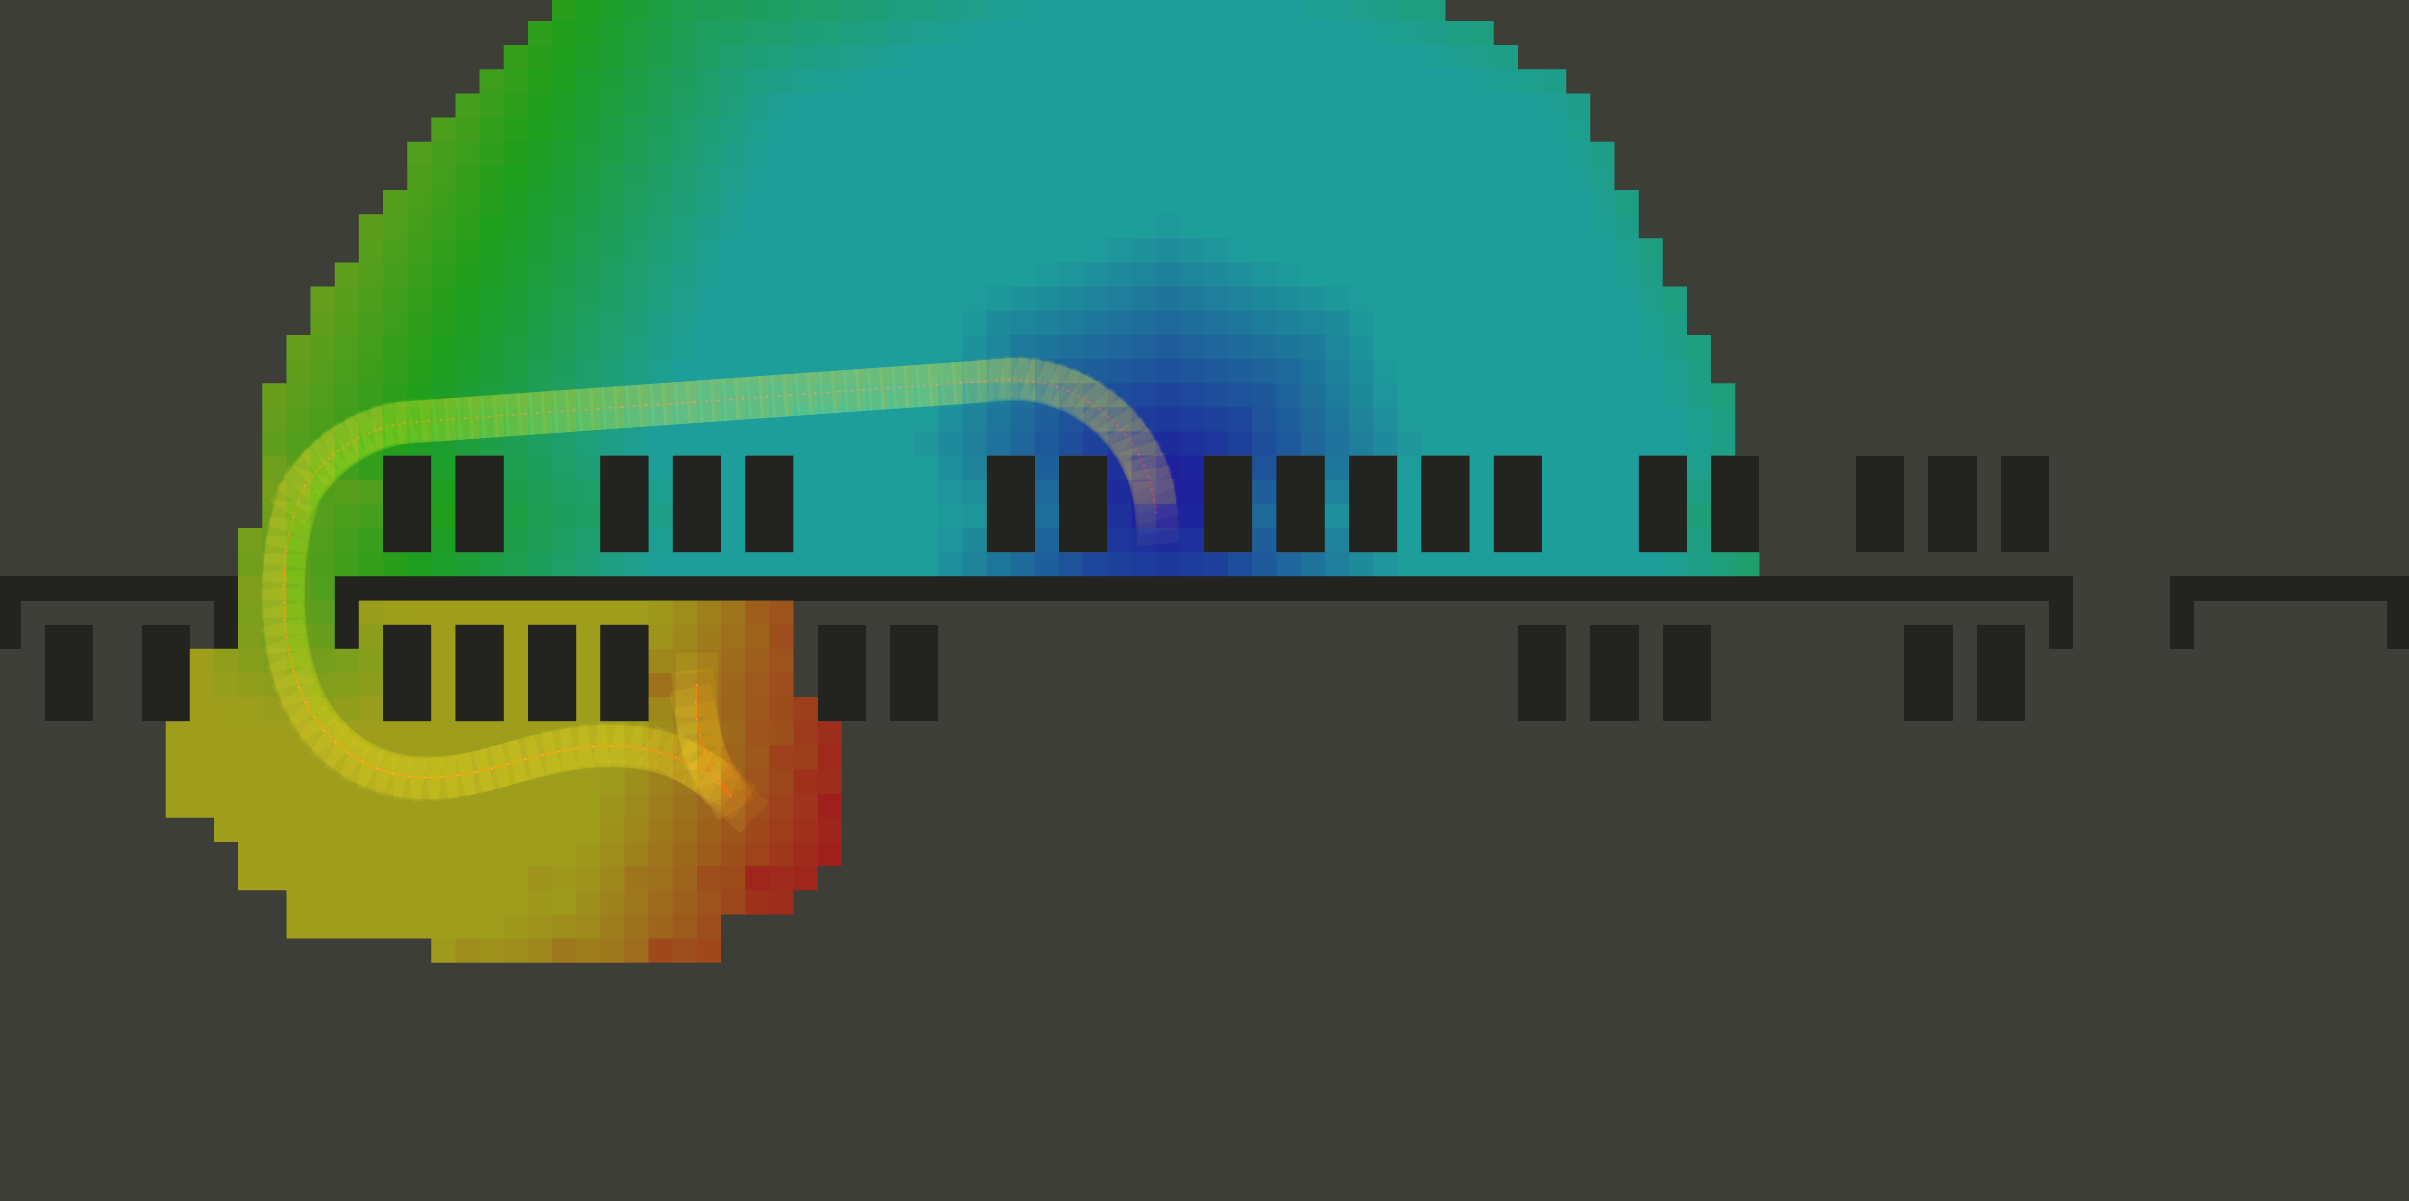
\includegraphics[width=\textwidth]{scenarioParking2dCost.png}
        \caption{2D A* \& Reeds Shepp, 4767 vertices (1517 vertices), length x\,m}
    \label{fig:scenarioParking2dCost}
    \end{subfigure}
    \caption{The parking structure scenario}
    \label{fig:scenarioParking}
\end{figure}

\subsection{Obstacles}
The size of the binary obstacle grid for the obstacles scenario is 50\,m $\times$ 100\,m. The environment is randomly scattered with quadratic obstacles of 1\,m and 2\,m width. The initial state $x_s$ as well as the goal $x_g$ both face towards the left.

\subsubsection{Analysis}
\Fref{fig:scenarioObstacles2d} shows the path found using the 2D A* heuristic. The search expands vertices in a more or less straight forward manner towards the goal. In roughly the middle of the grid the analytical expansion finds a solution and connects collision free to the goal.

Adding the Dubins heuristic in \Fref{fig:scenarioObstacles2dDubins} the search expands less vertices at the beginning, especially less reversing states. Afterwards the search continues towards the goal but not using the shortest Euclidean path. Much later than 2D A* the search ends due to a successful analytical expansion.

Using the Reeds Shepp heuristic, in \Fref{fig:scenarioObstacles2dReedsShepp} the search searches a much larger amount of states in the vicinity of the initial state. While the search progresses towards the goal, it is noticeable that the search expands states in a circular fashion along the path, until the analytical expansion connects to the goal.

\subsubsection{Discussion}
Since the 2D A* heuristic does not account for the non-holonomic constrains of the vehicle it guides the search similar as a Euclidean heuristic would straight to the goal until the Dubins path of the analytical expansion corrects for the behavior. The Dubins heuristic expands nodes keeping the goal heading of the vehicle in mind, essentially restricting the search to an area along a Dubins curve. While the heuristic expands much more nodes than the 2D A* only version, this is due to the fact, that obstacles continuously block a direct connection for the path chosen by the Dubins heuristic. Only at last the analytical expansion succeeds. For the Reeds Shepp heuristic the case behaves slightly different. Since the heuristic calculates the cost under the assumption that the vehicle can drive in both directions it allows for much more reverse states to be expanded. Along the path towards the goal the Reeds Shepp heuristic continuously tries to change the heading of the car by expanding states that deviate from the path in a circular fashion.

\begin{figure}[h]
    \centering
    \begin{subfigure}[t]{\textwidth}
        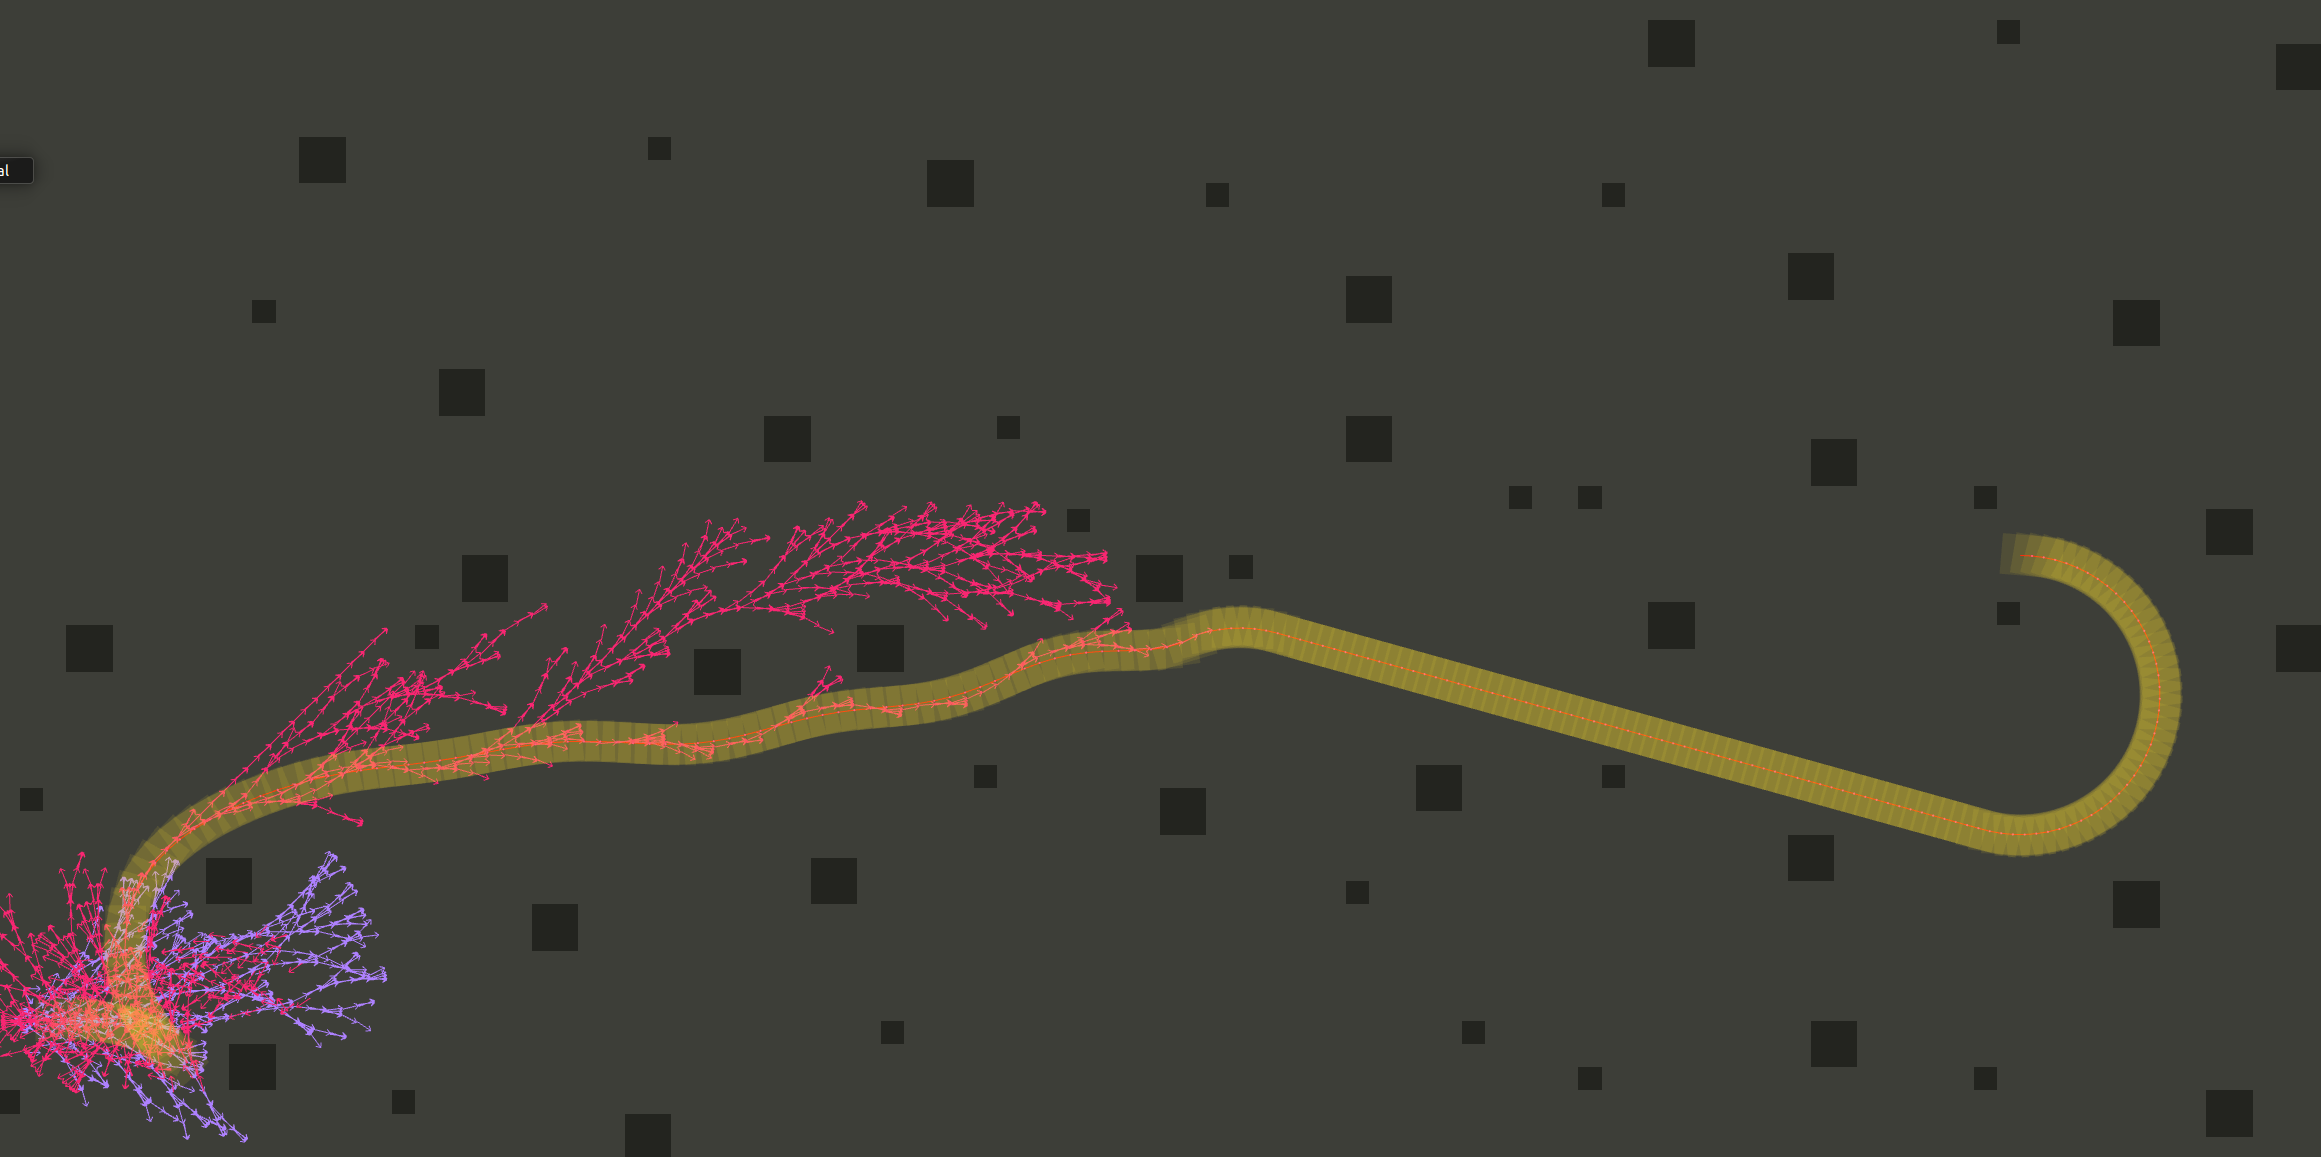
\includegraphics[width=\textwidth]{scenarioObstacles2d.png}
        \caption{2D A*, 2685 vertices, length 116.882\,m}
        \label{fig:scenarioObstacles2d}
    \end{subfigure}
    \begin{subfigure}[t]{\textwidth}
        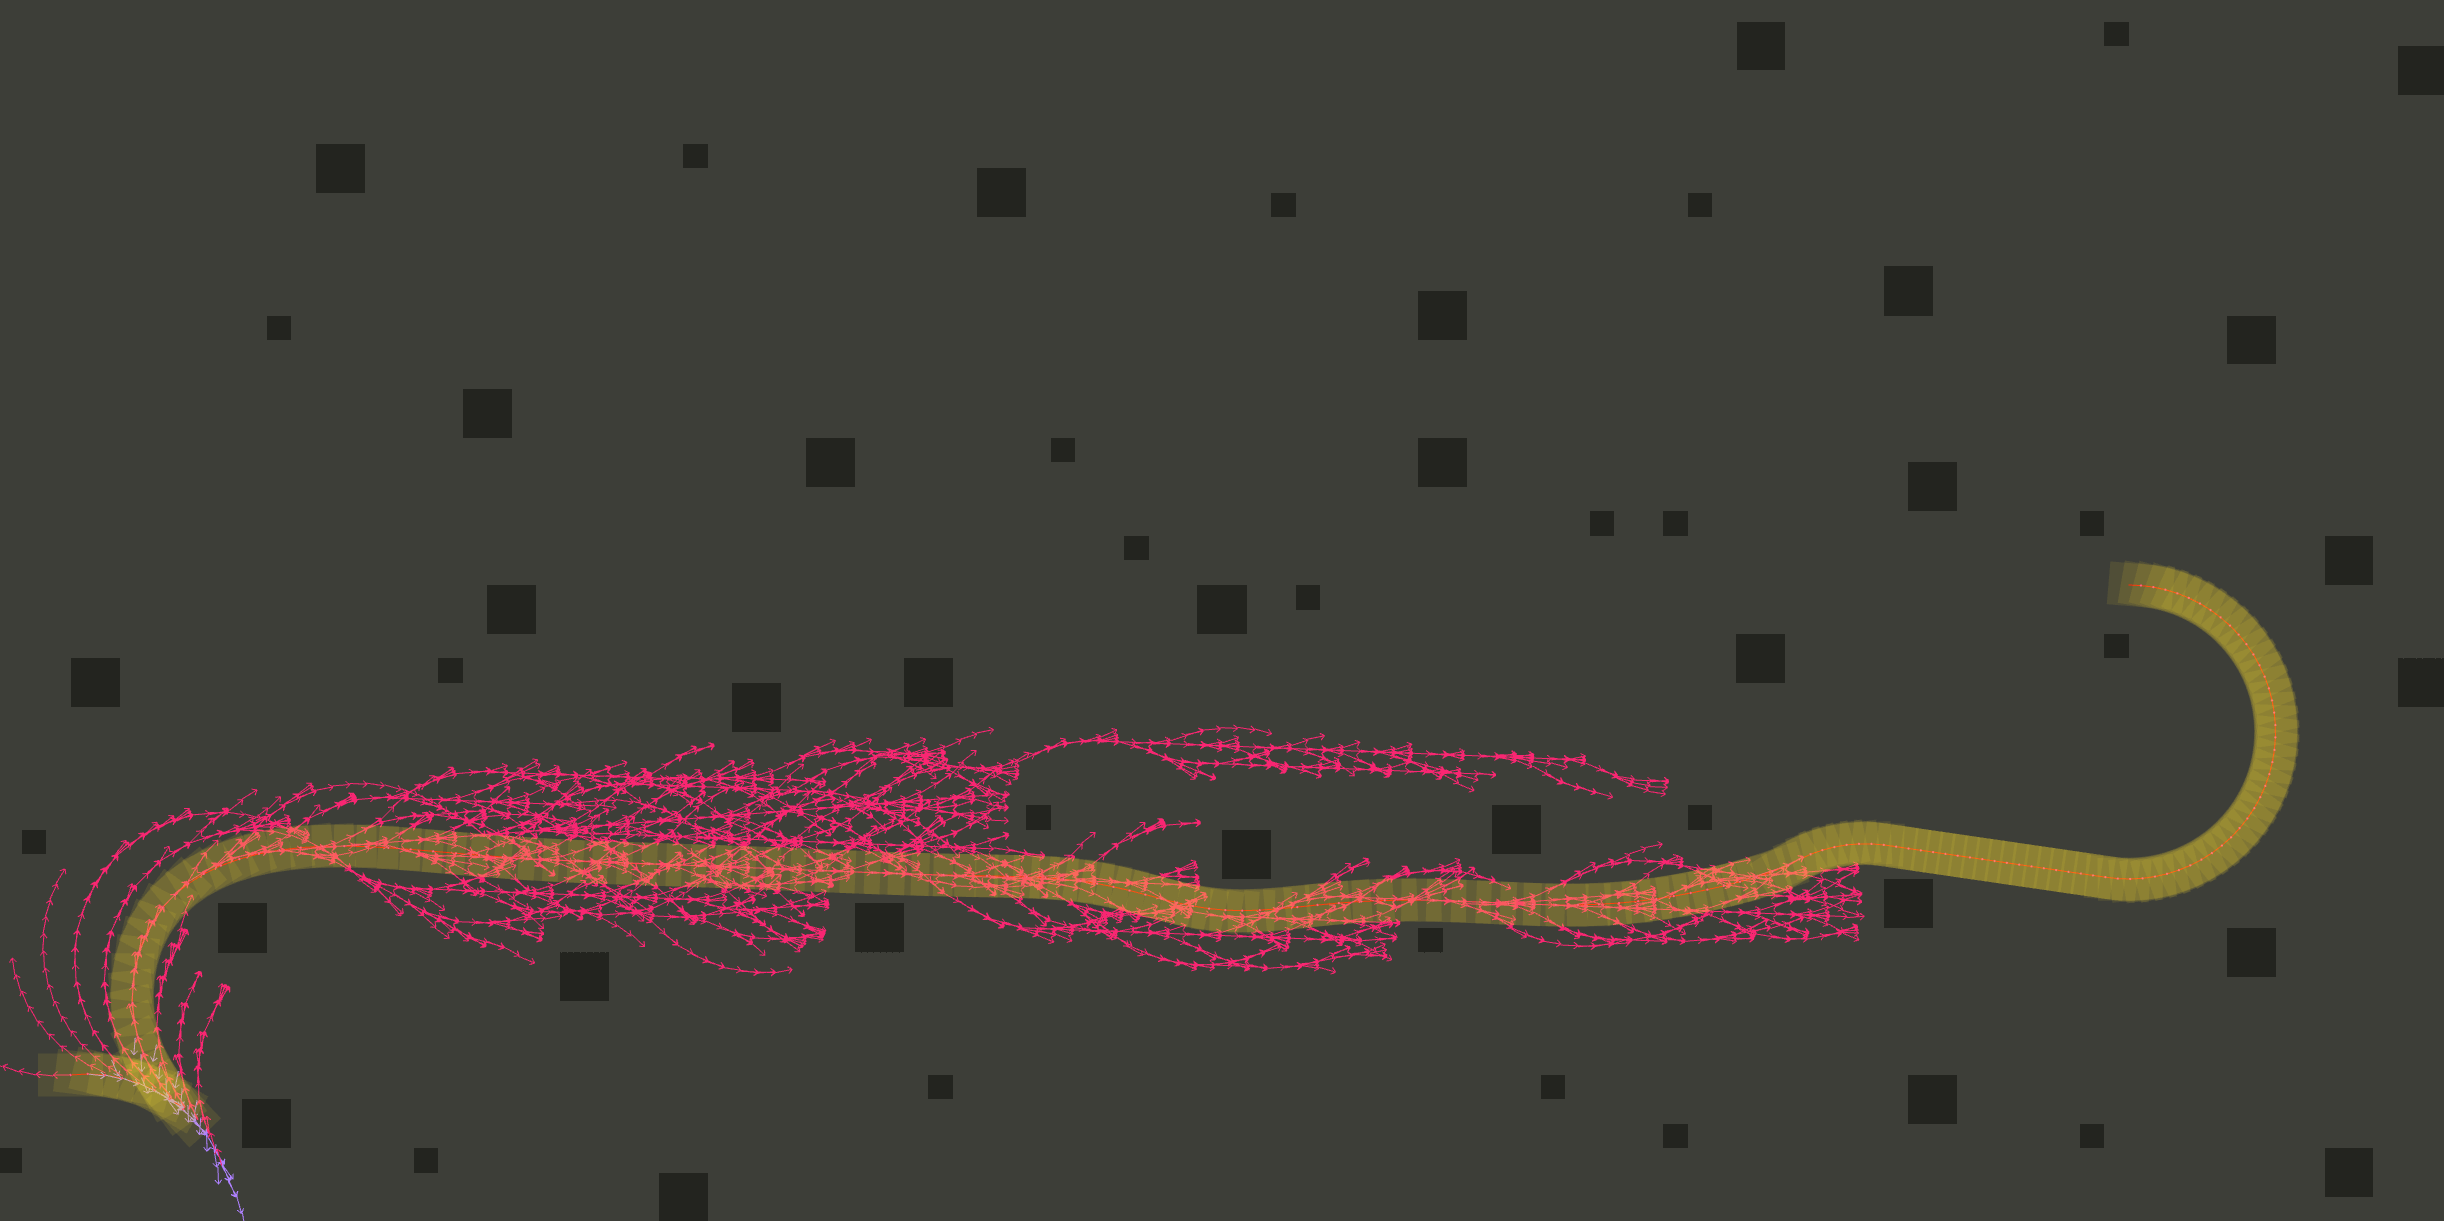
\includegraphics[width=\textwidth]{scenarioObstacles2dDubins.png}
        \caption{2D A* \& Dubins, 3486 vertices, length 114.961\,m}
        \label{fig:scenarioObstacles2dDubins}
    \end{subfigure}    
    \begin{subfigure}[t]{\textwidth}
        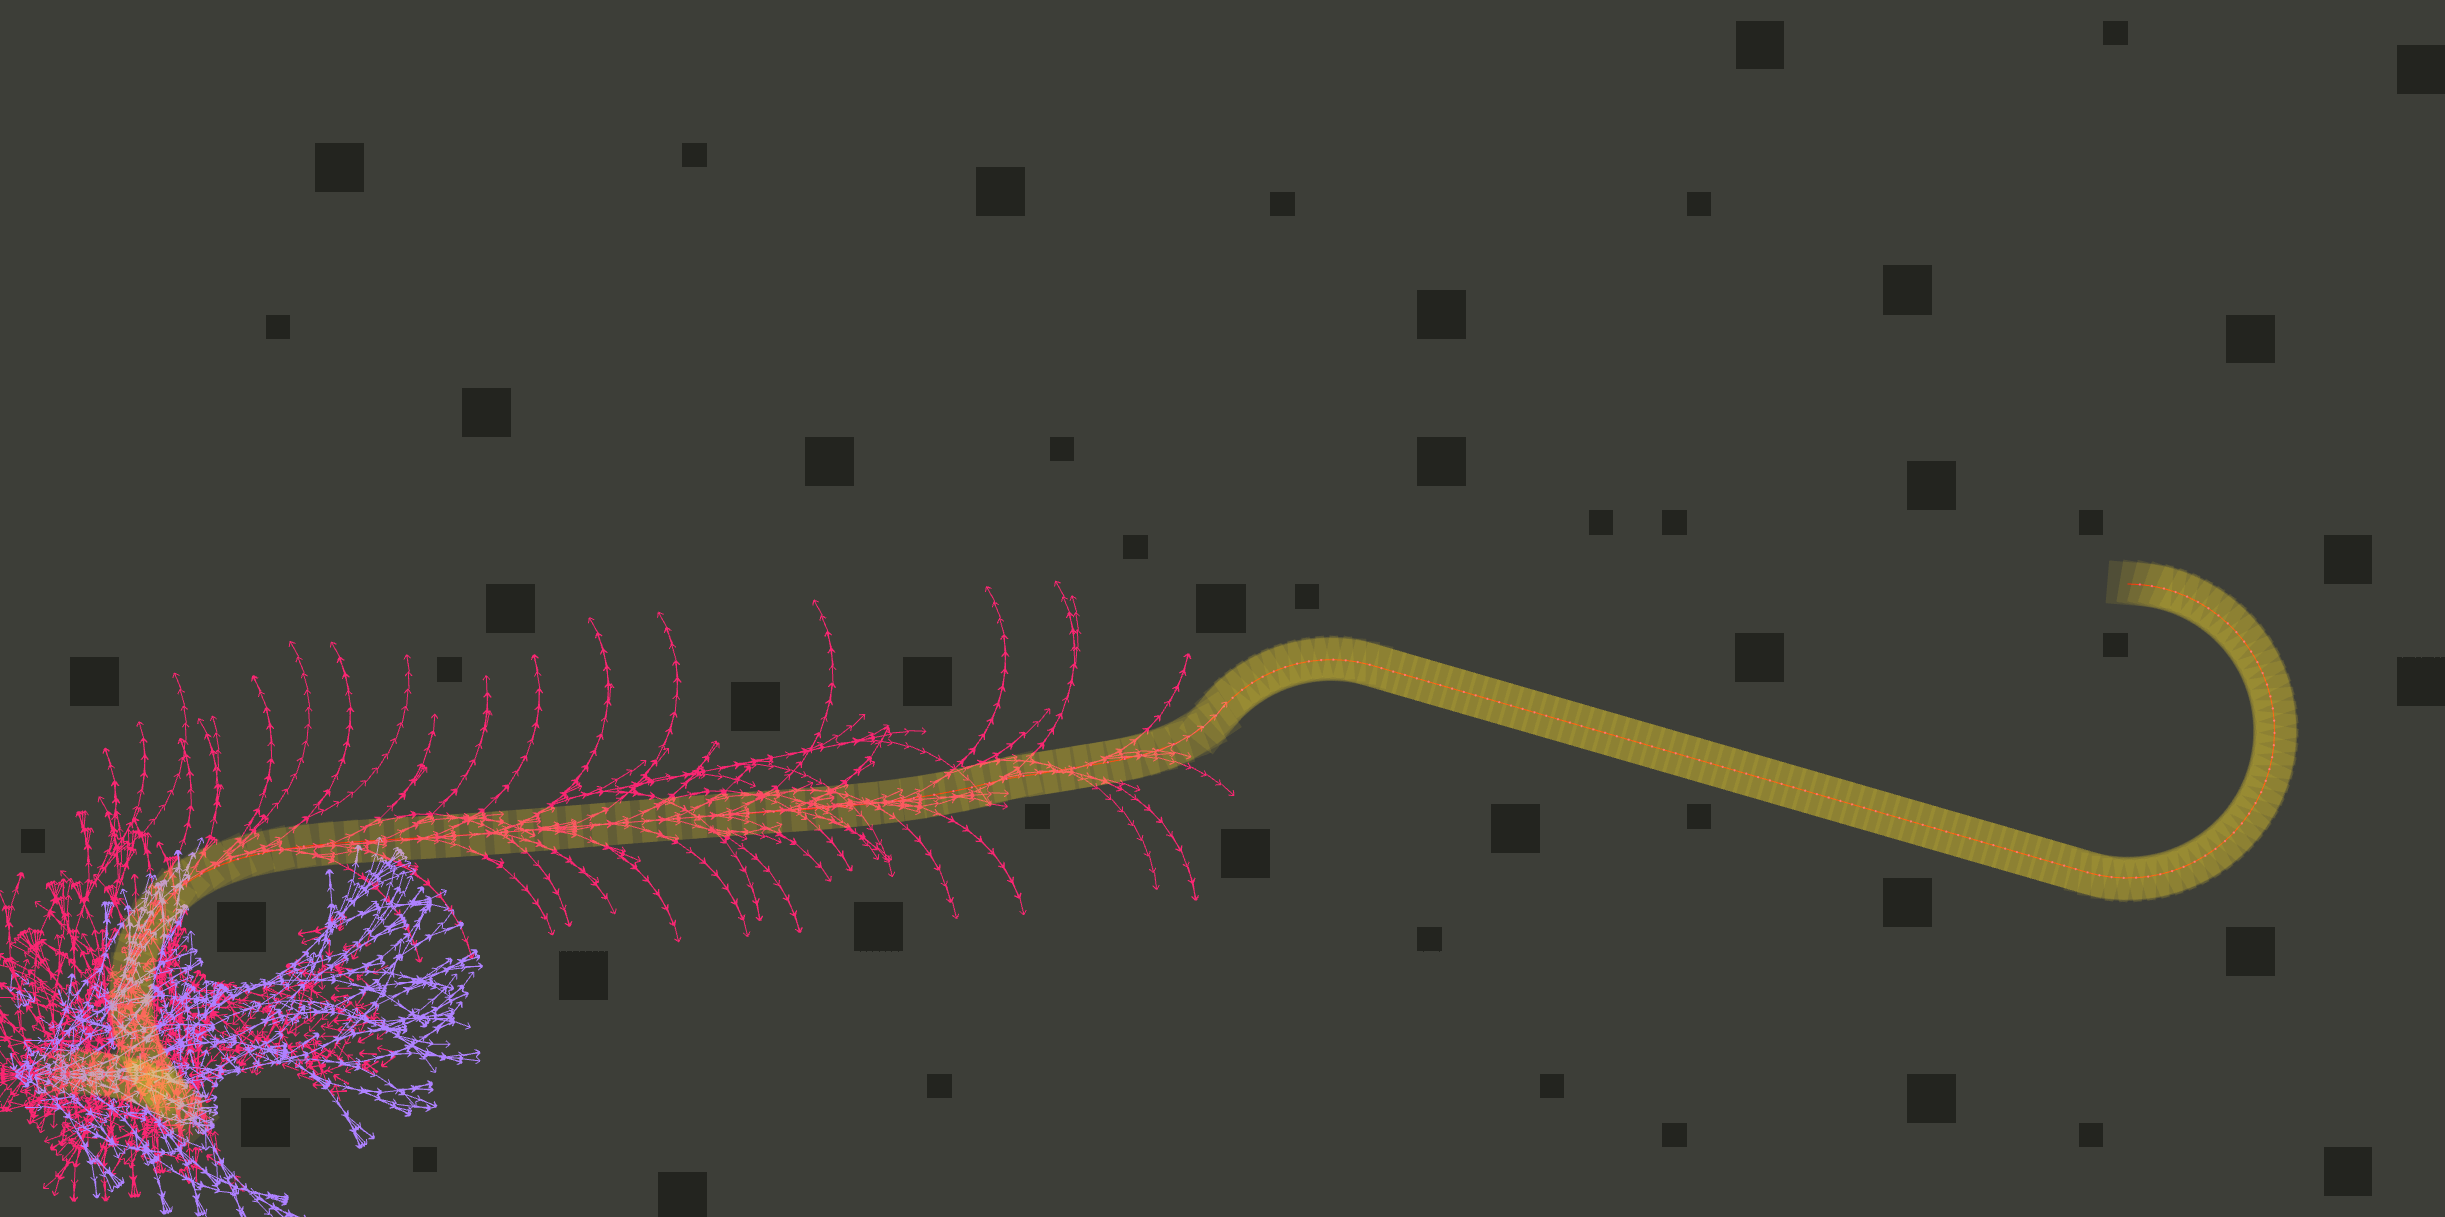
\includegraphics[width=\textwidth]{scenarioObstacles2dReedsShepp.png}
        \caption{2D A* \& Reeds Shepp, 4316 vertices, length 116.647\,m}
        \label{fig:scenarioObstacles2dReedsShepp}
    \end{subfigure}
%    \begin{subfigure}[t]{\textwidth}
%        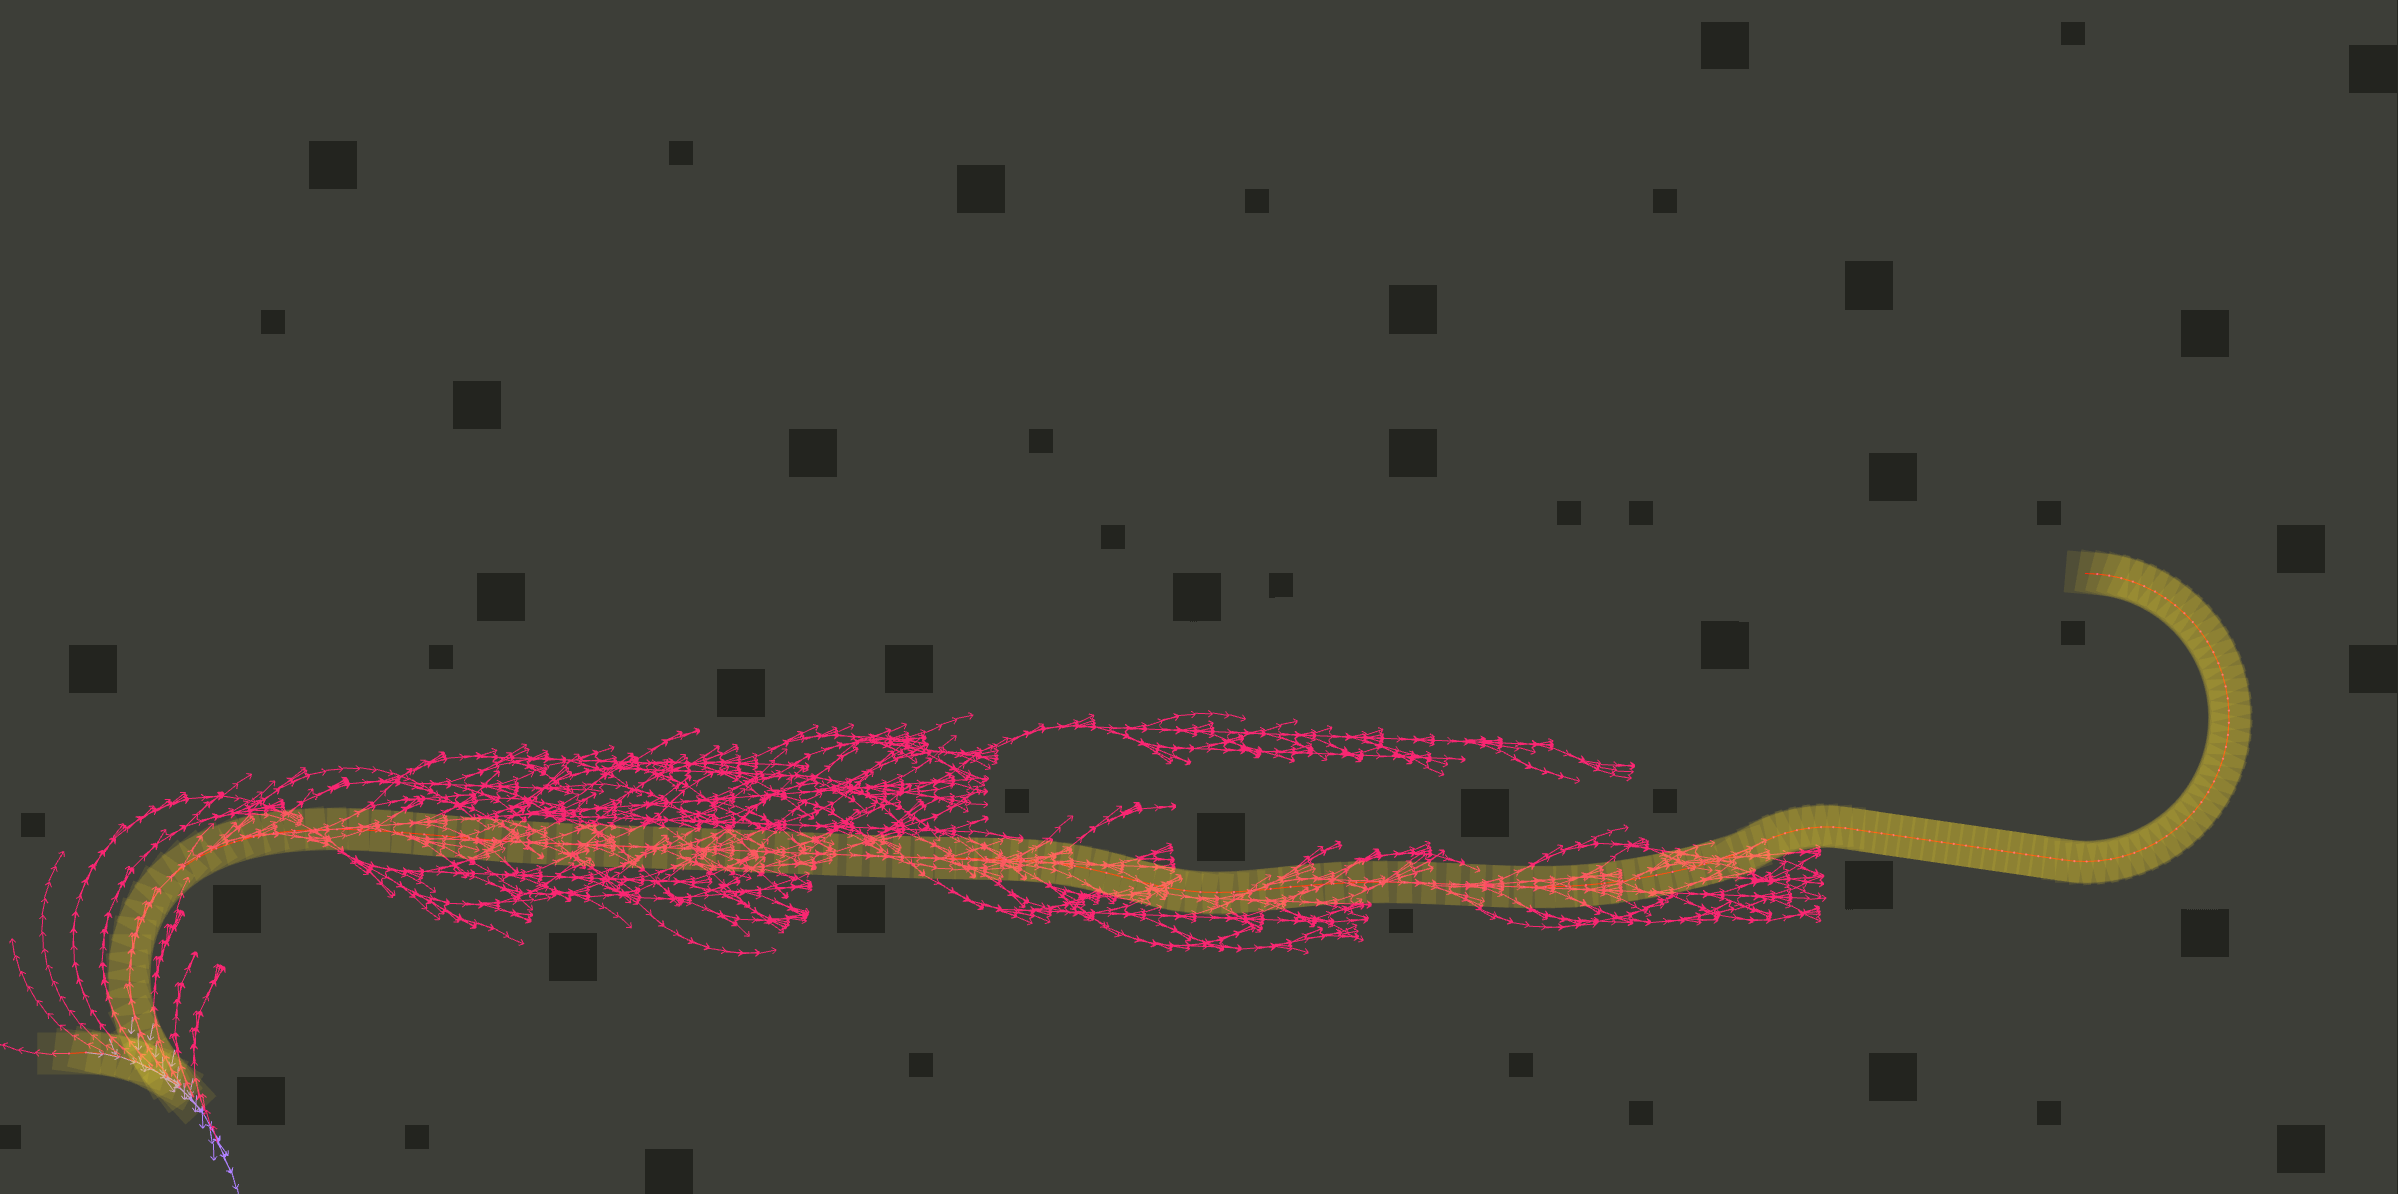
\includegraphics[width=\textwidth]{scenarioObstaclesDubins.png}
%        \caption{Dubins, 3486 vertices, length 114.961\,m}
%        \label{fig:scenarioObstaclesDubins}
%    \end{subfigure}
%    \begin{subfigure}[t]{\textwidth}
%        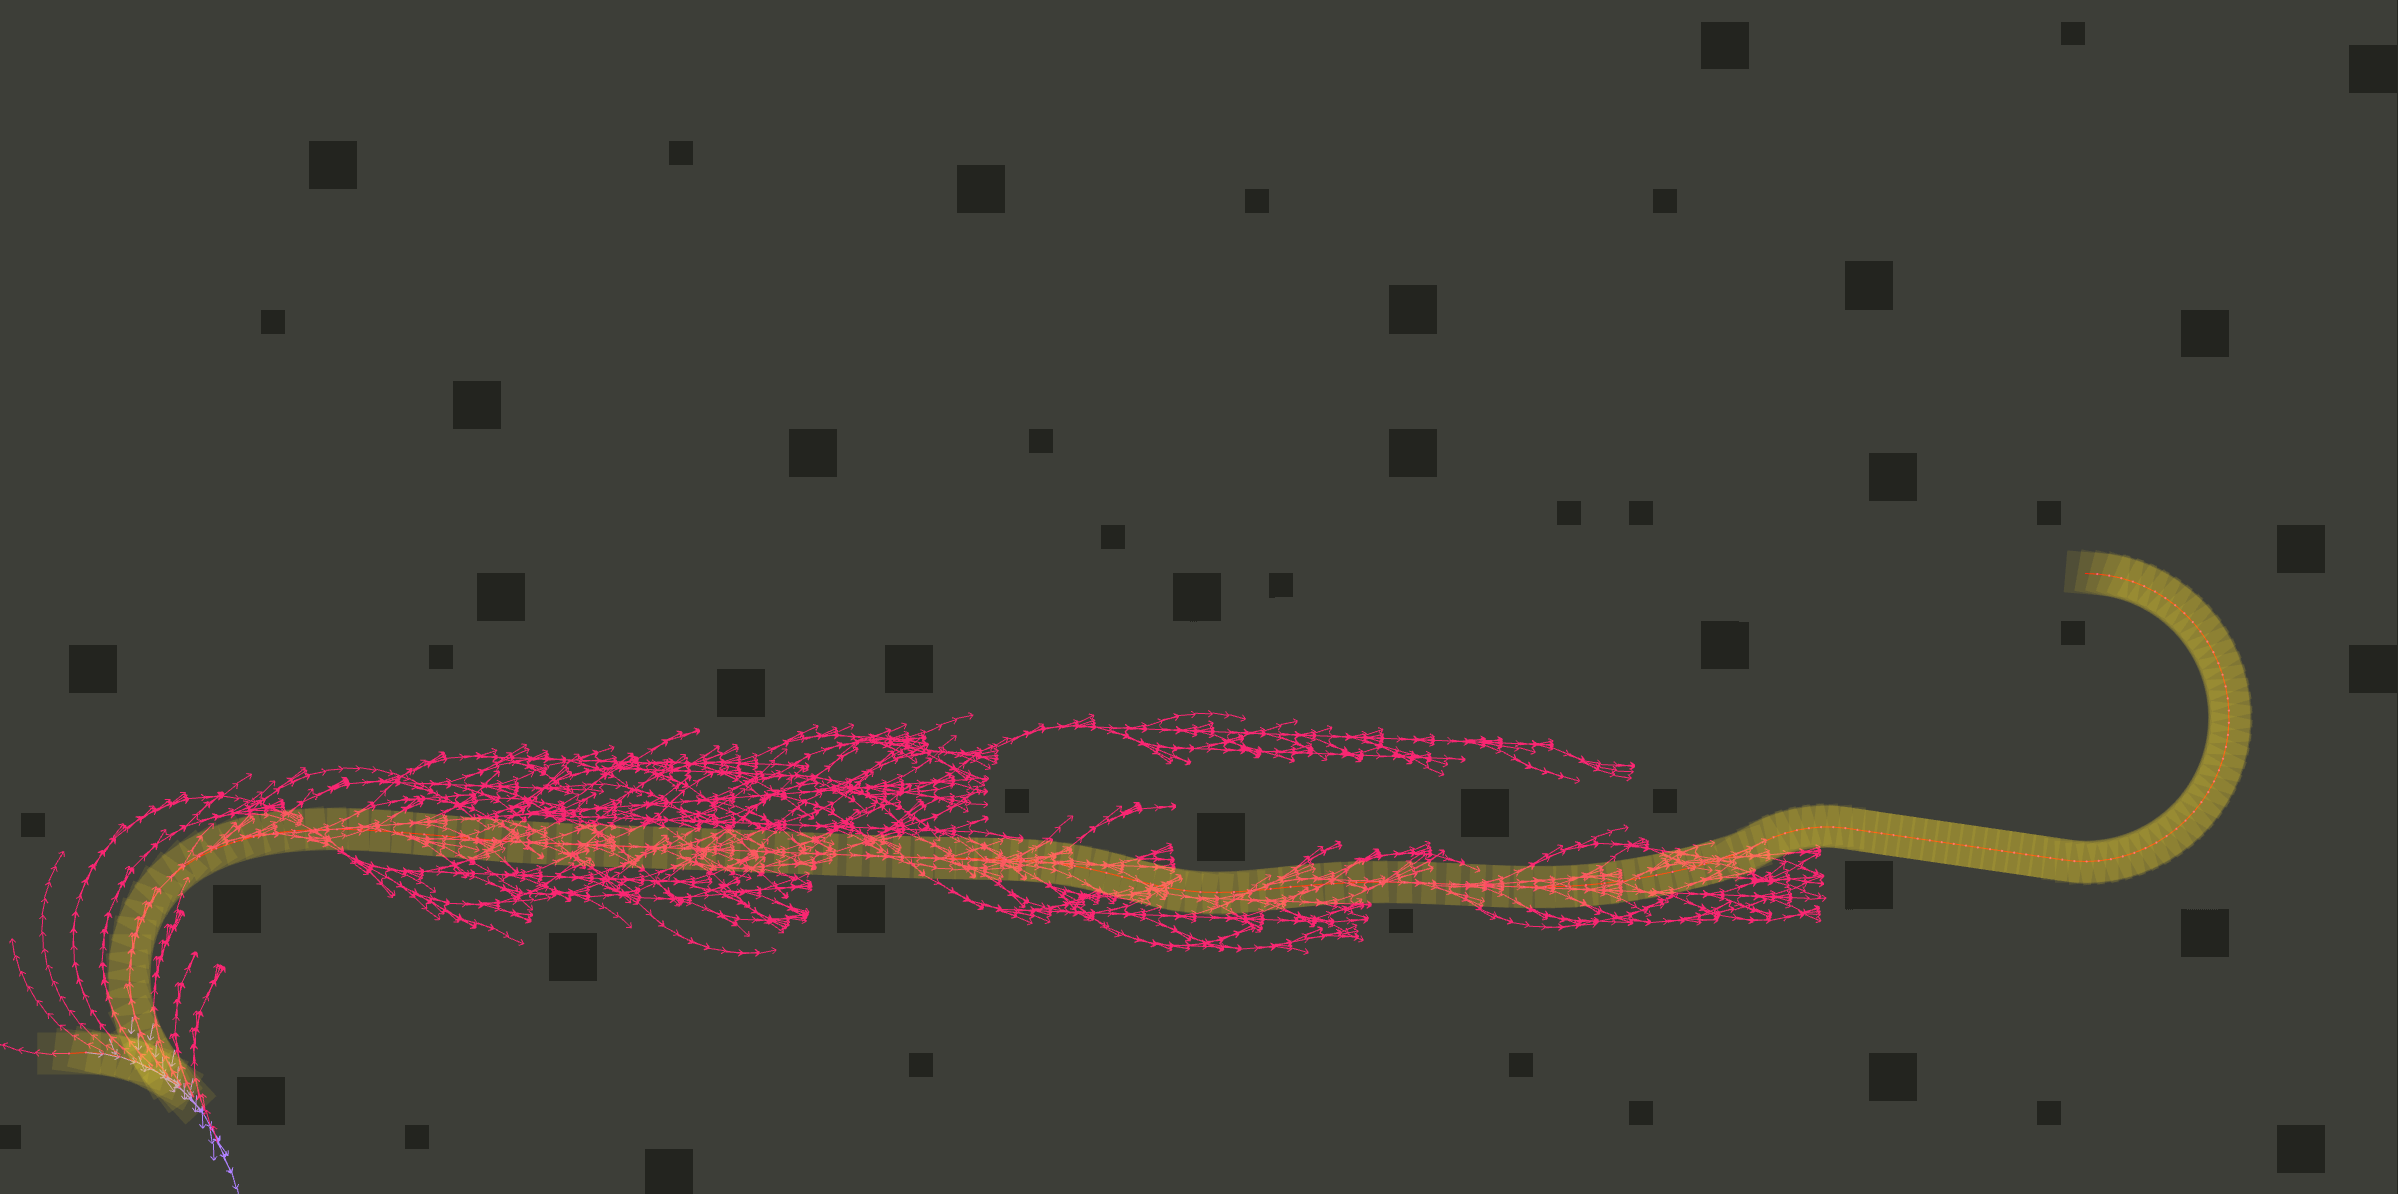
\includegraphics[width=\textwidth]{scenarioObstaclesDubins.png}
%        \caption{Reeds Shepp, 3486 vertices, length 116.141\,m}
%        \label{fig:scenarioObstaclesDubins}
%    \end{subfigure}
    \caption{The obstacle scenario}
    \label{fig:scenarioObstacle}
\end{figure}

\subsection{Wall}

\begin{figure}[h]
    \centering
    \begin{subfigure}[t]{\textwidth}
        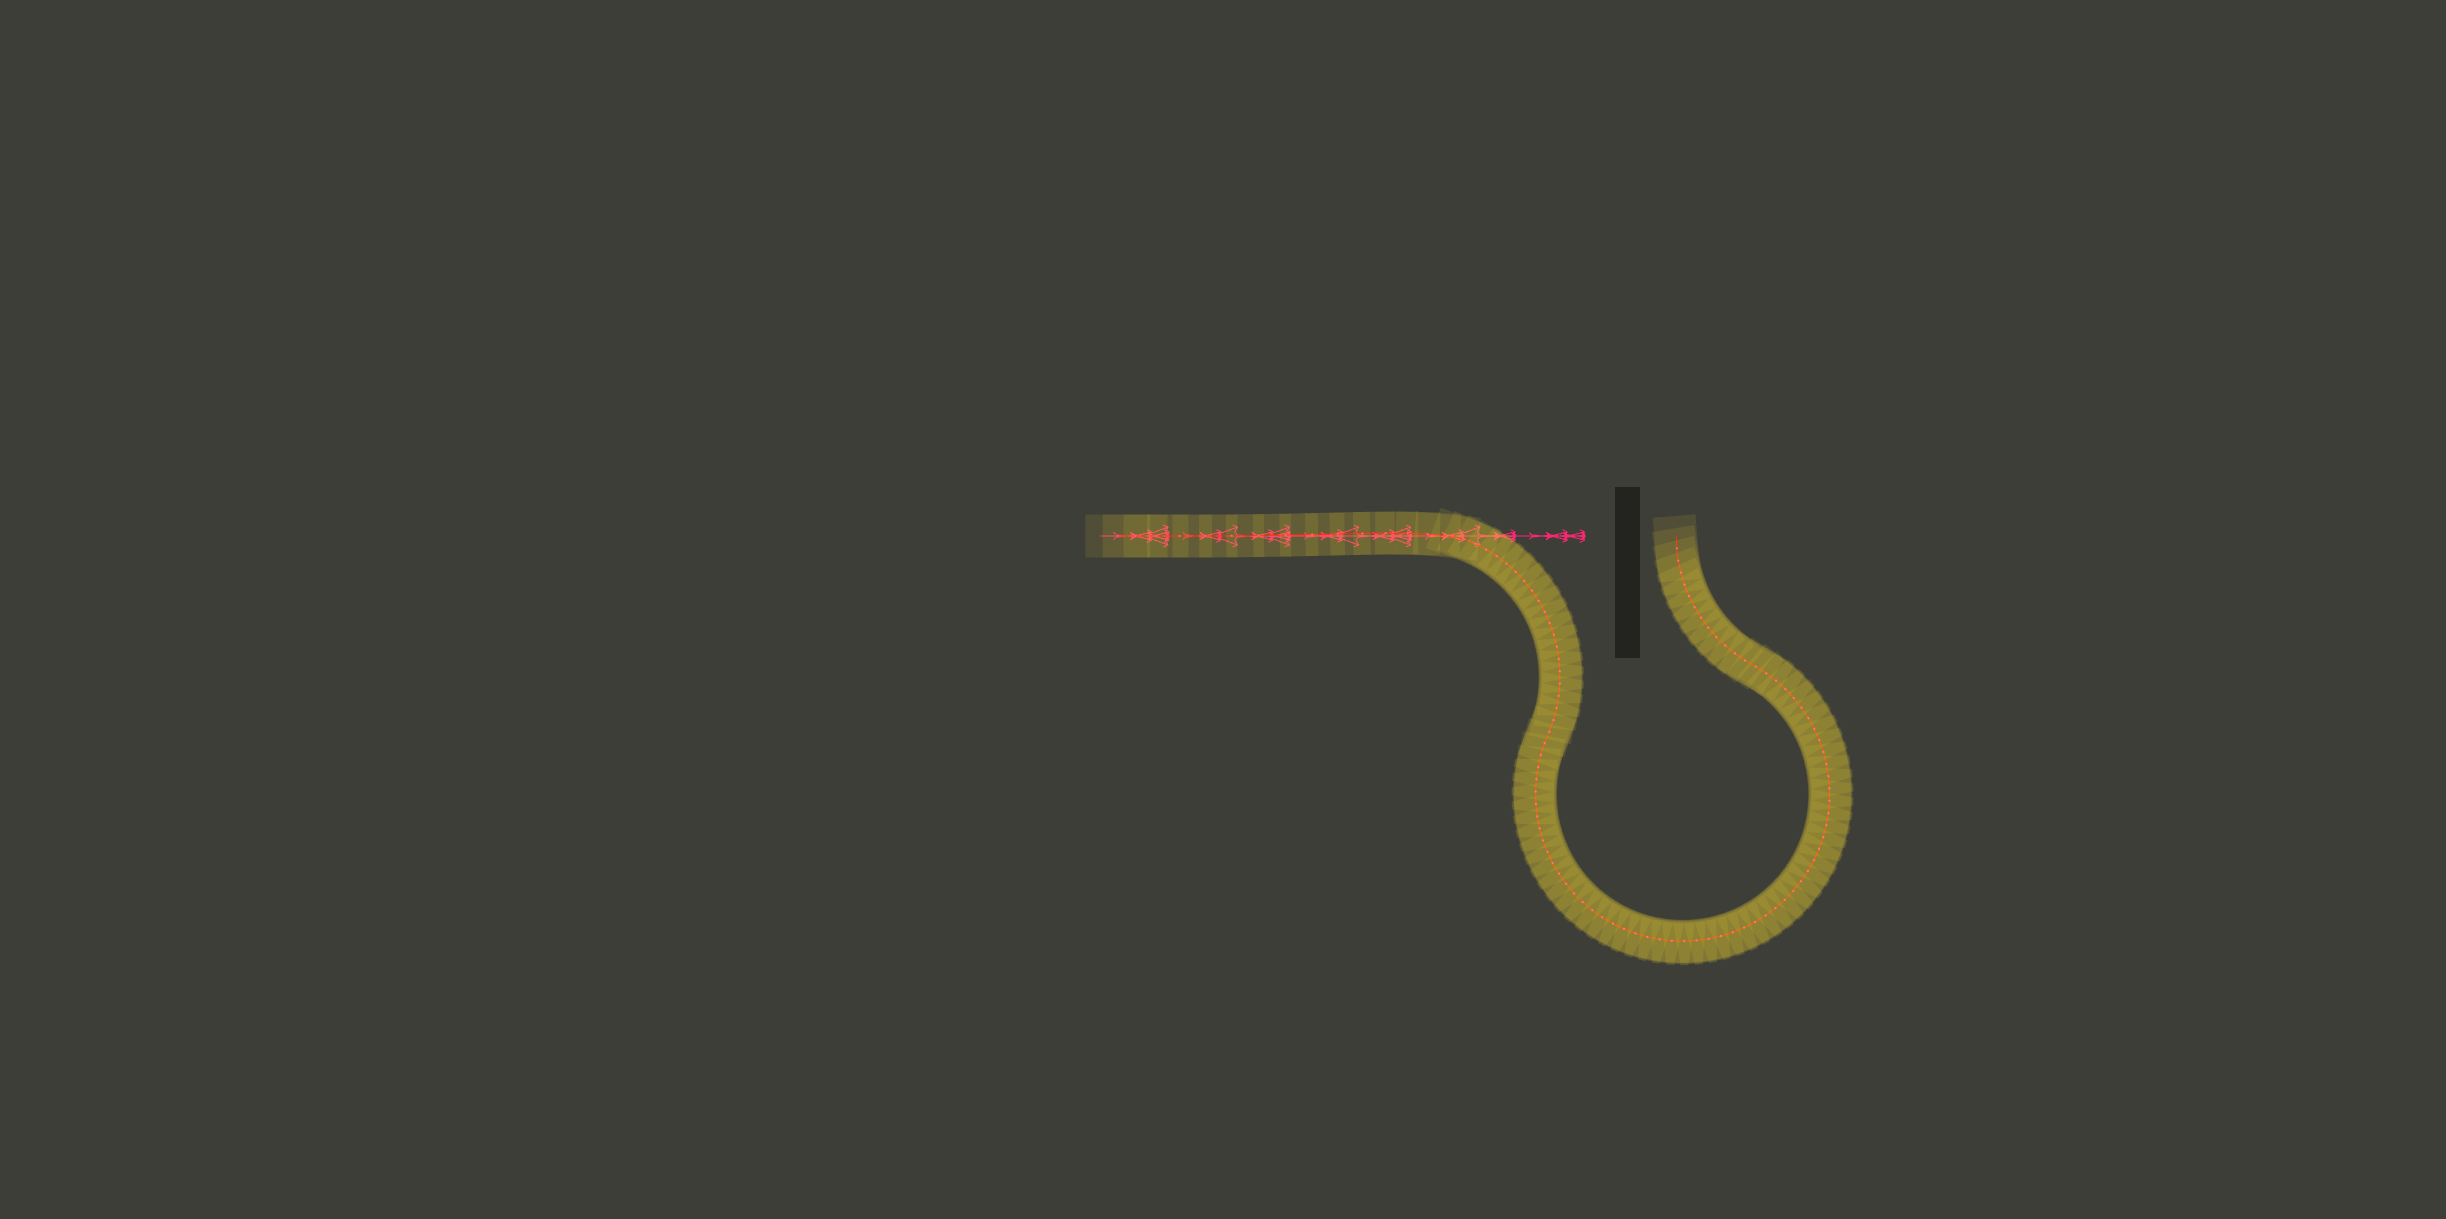
\includegraphics[width=\textwidth]{scenarioWall.png}
        \caption{Euclidean, 237 vertices, length 58.224,m}
        \label{fig:scenarioWall}
    \end{subfigure}
    \begin{subfigure}[t]{\textwidth}
        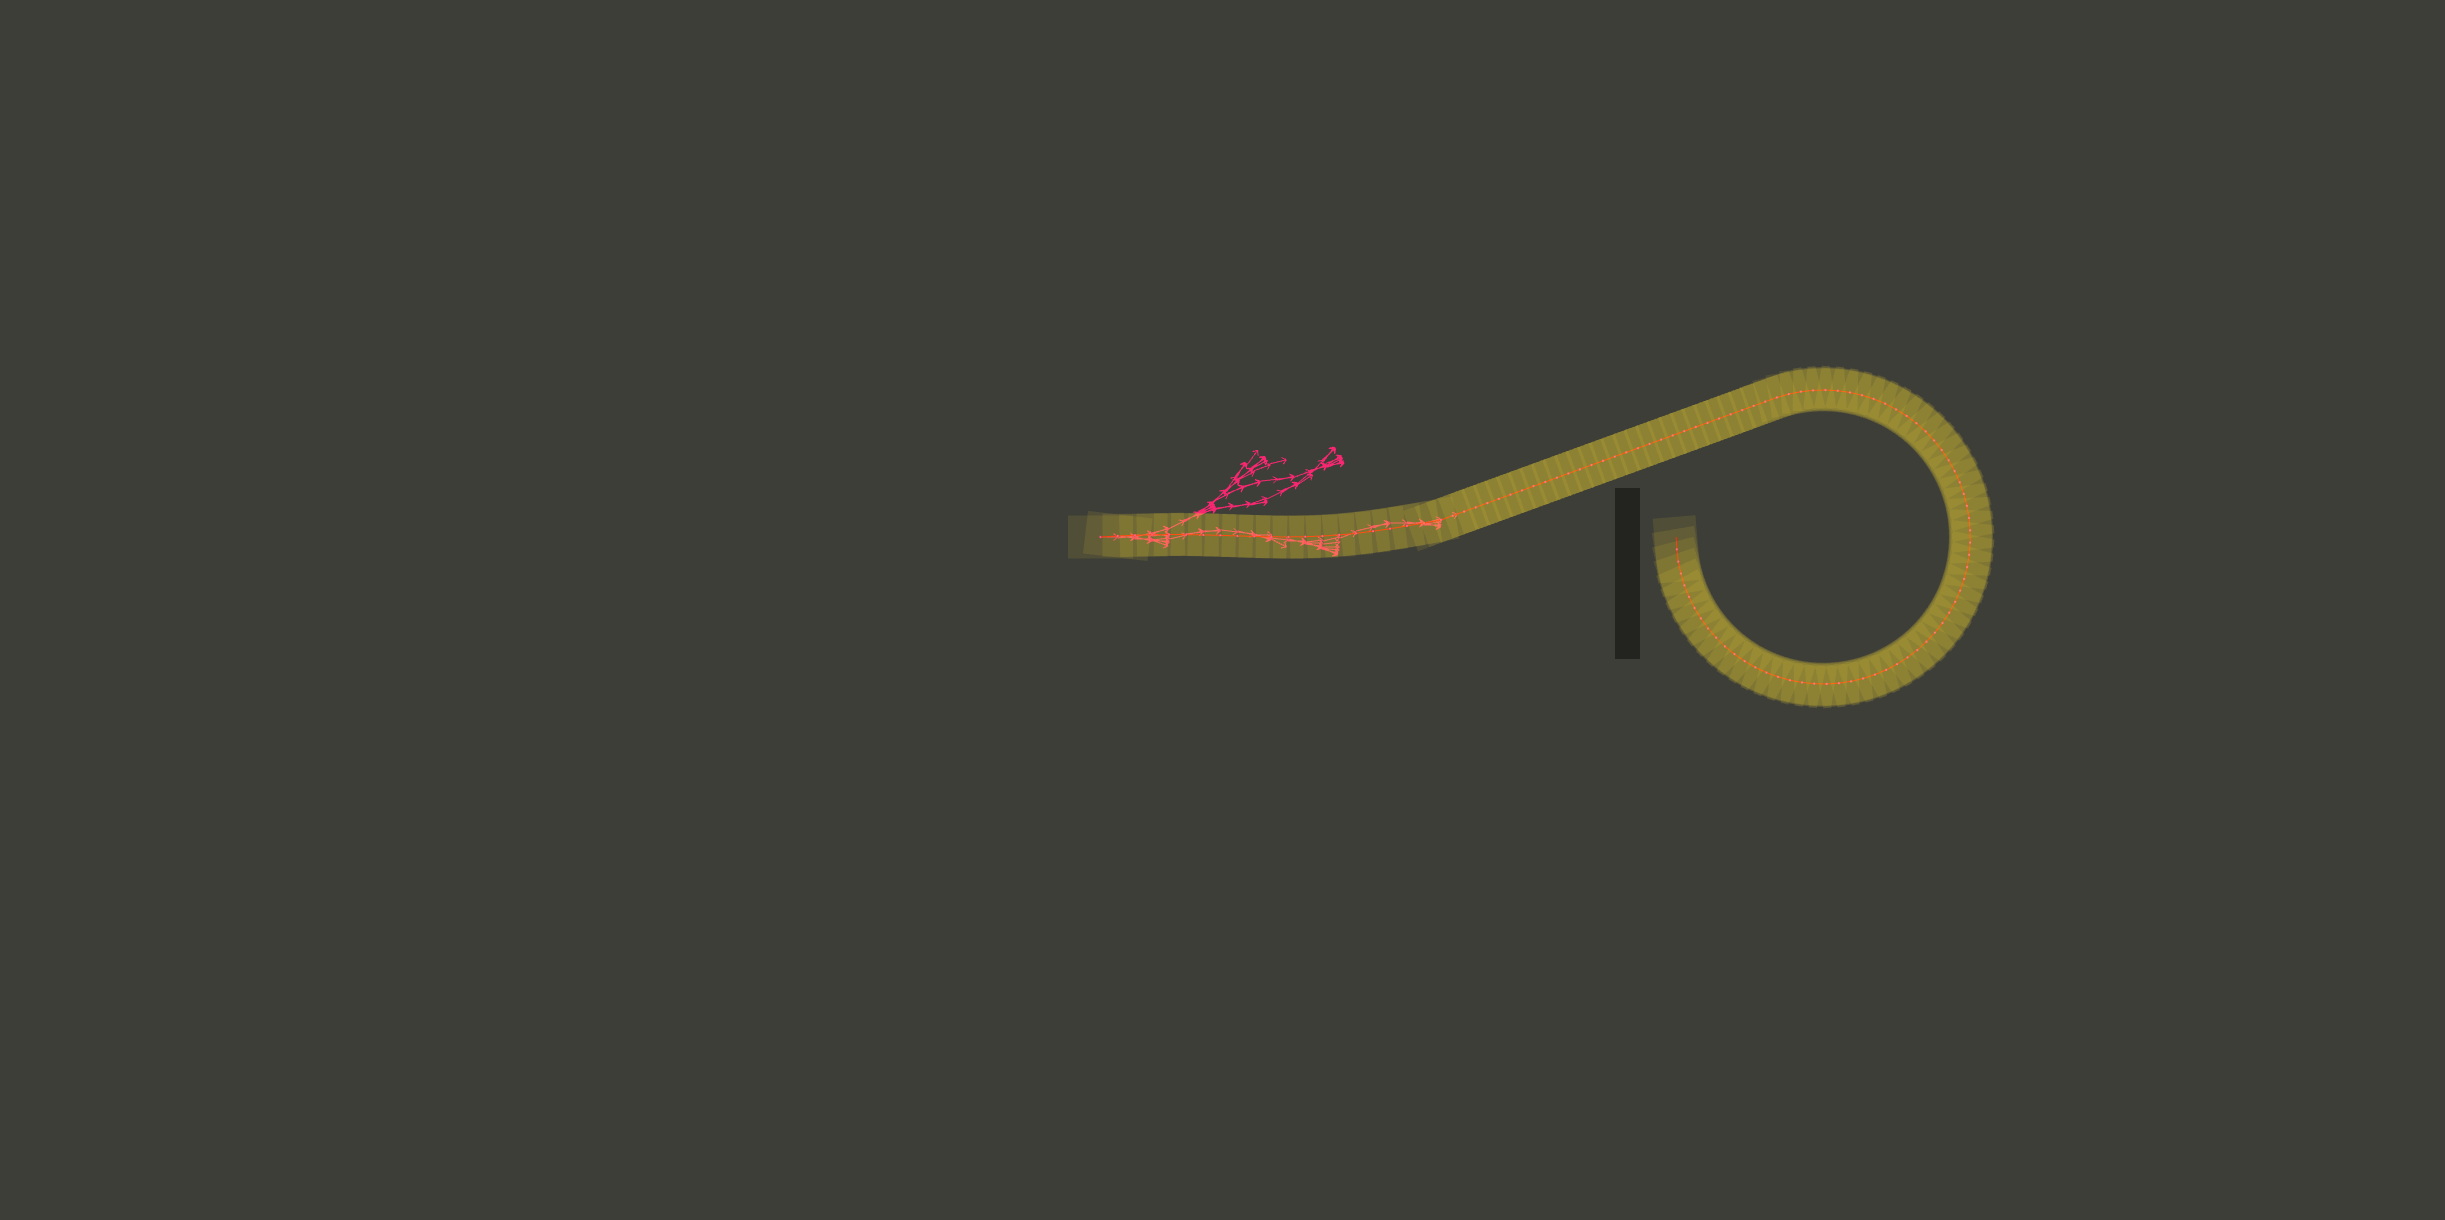
\includegraphics[width=\textwidth]{scenarioWall2d.png}
        \caption{2D A*, 129 vertices, length 58.914\,m}
        \label{fig:scenarioWall2d}
    \end{subfigure}    
    \begin{subfigure}[t]{\textwidth}
        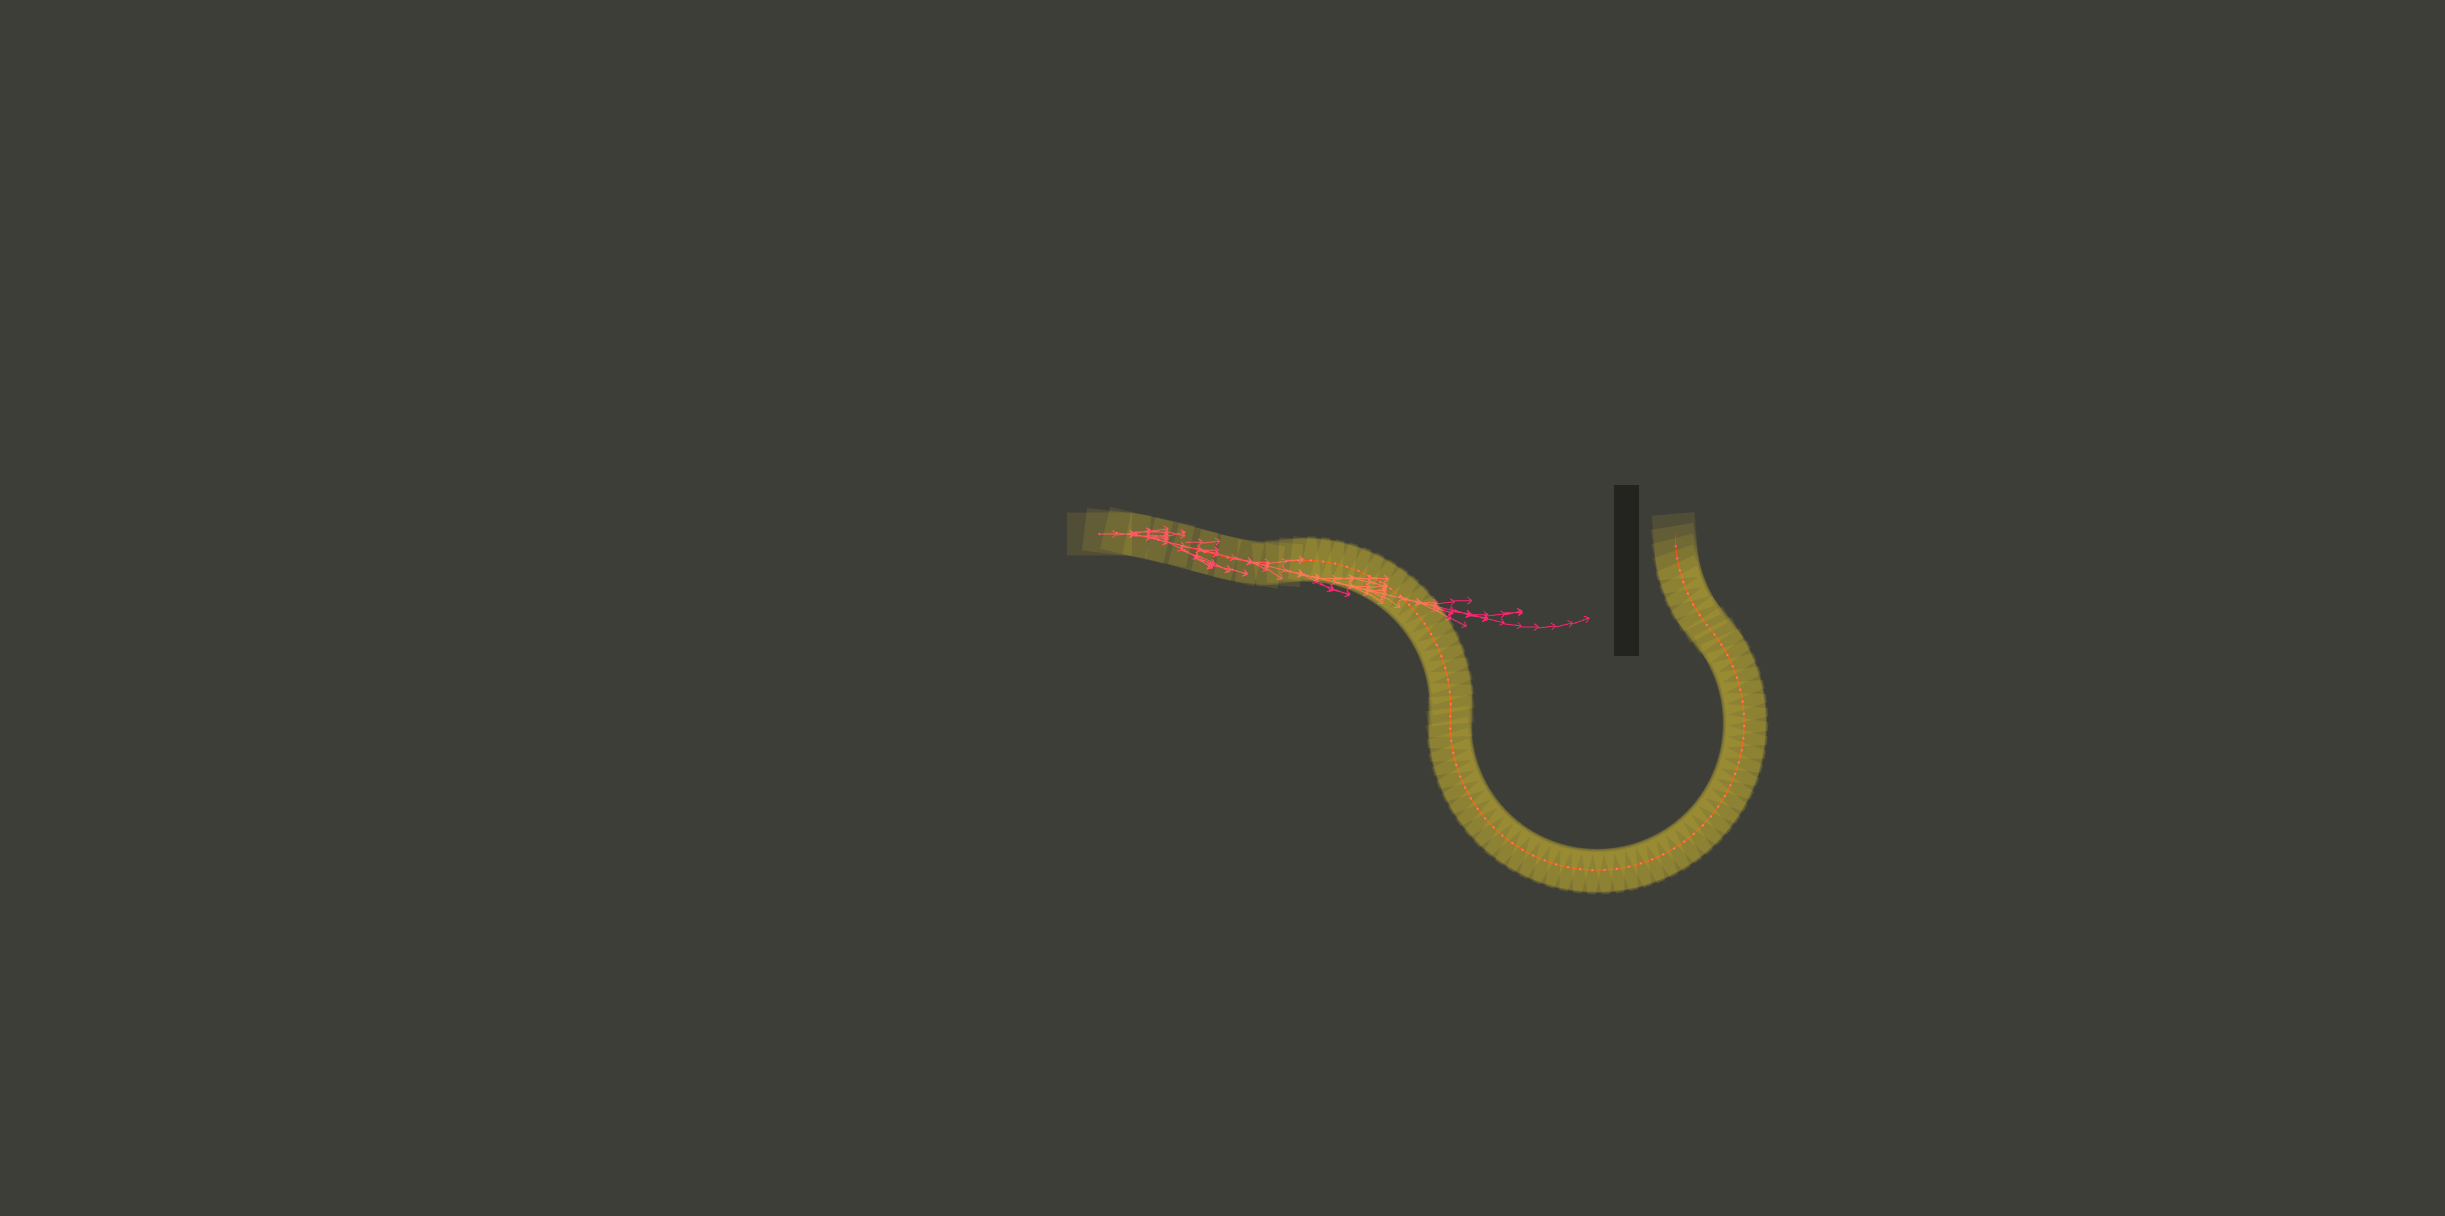
\includegraphics[width=\textwidth]{scenarioWallReedsShepp.png}
        \caption{Reeds Shepp, 124 vertices, length 45.780\,m}
        \label{fig:scenarioWallReedsShepp}
    \end{subfigure}
    \caption{The wall scenario}
    \label{fig:scenarioWall}
\end{figure}

\subsection{Dead End}

\begin{figure}[h]
    \centering
    \begin{subfigure}[t]{\textwidth}
        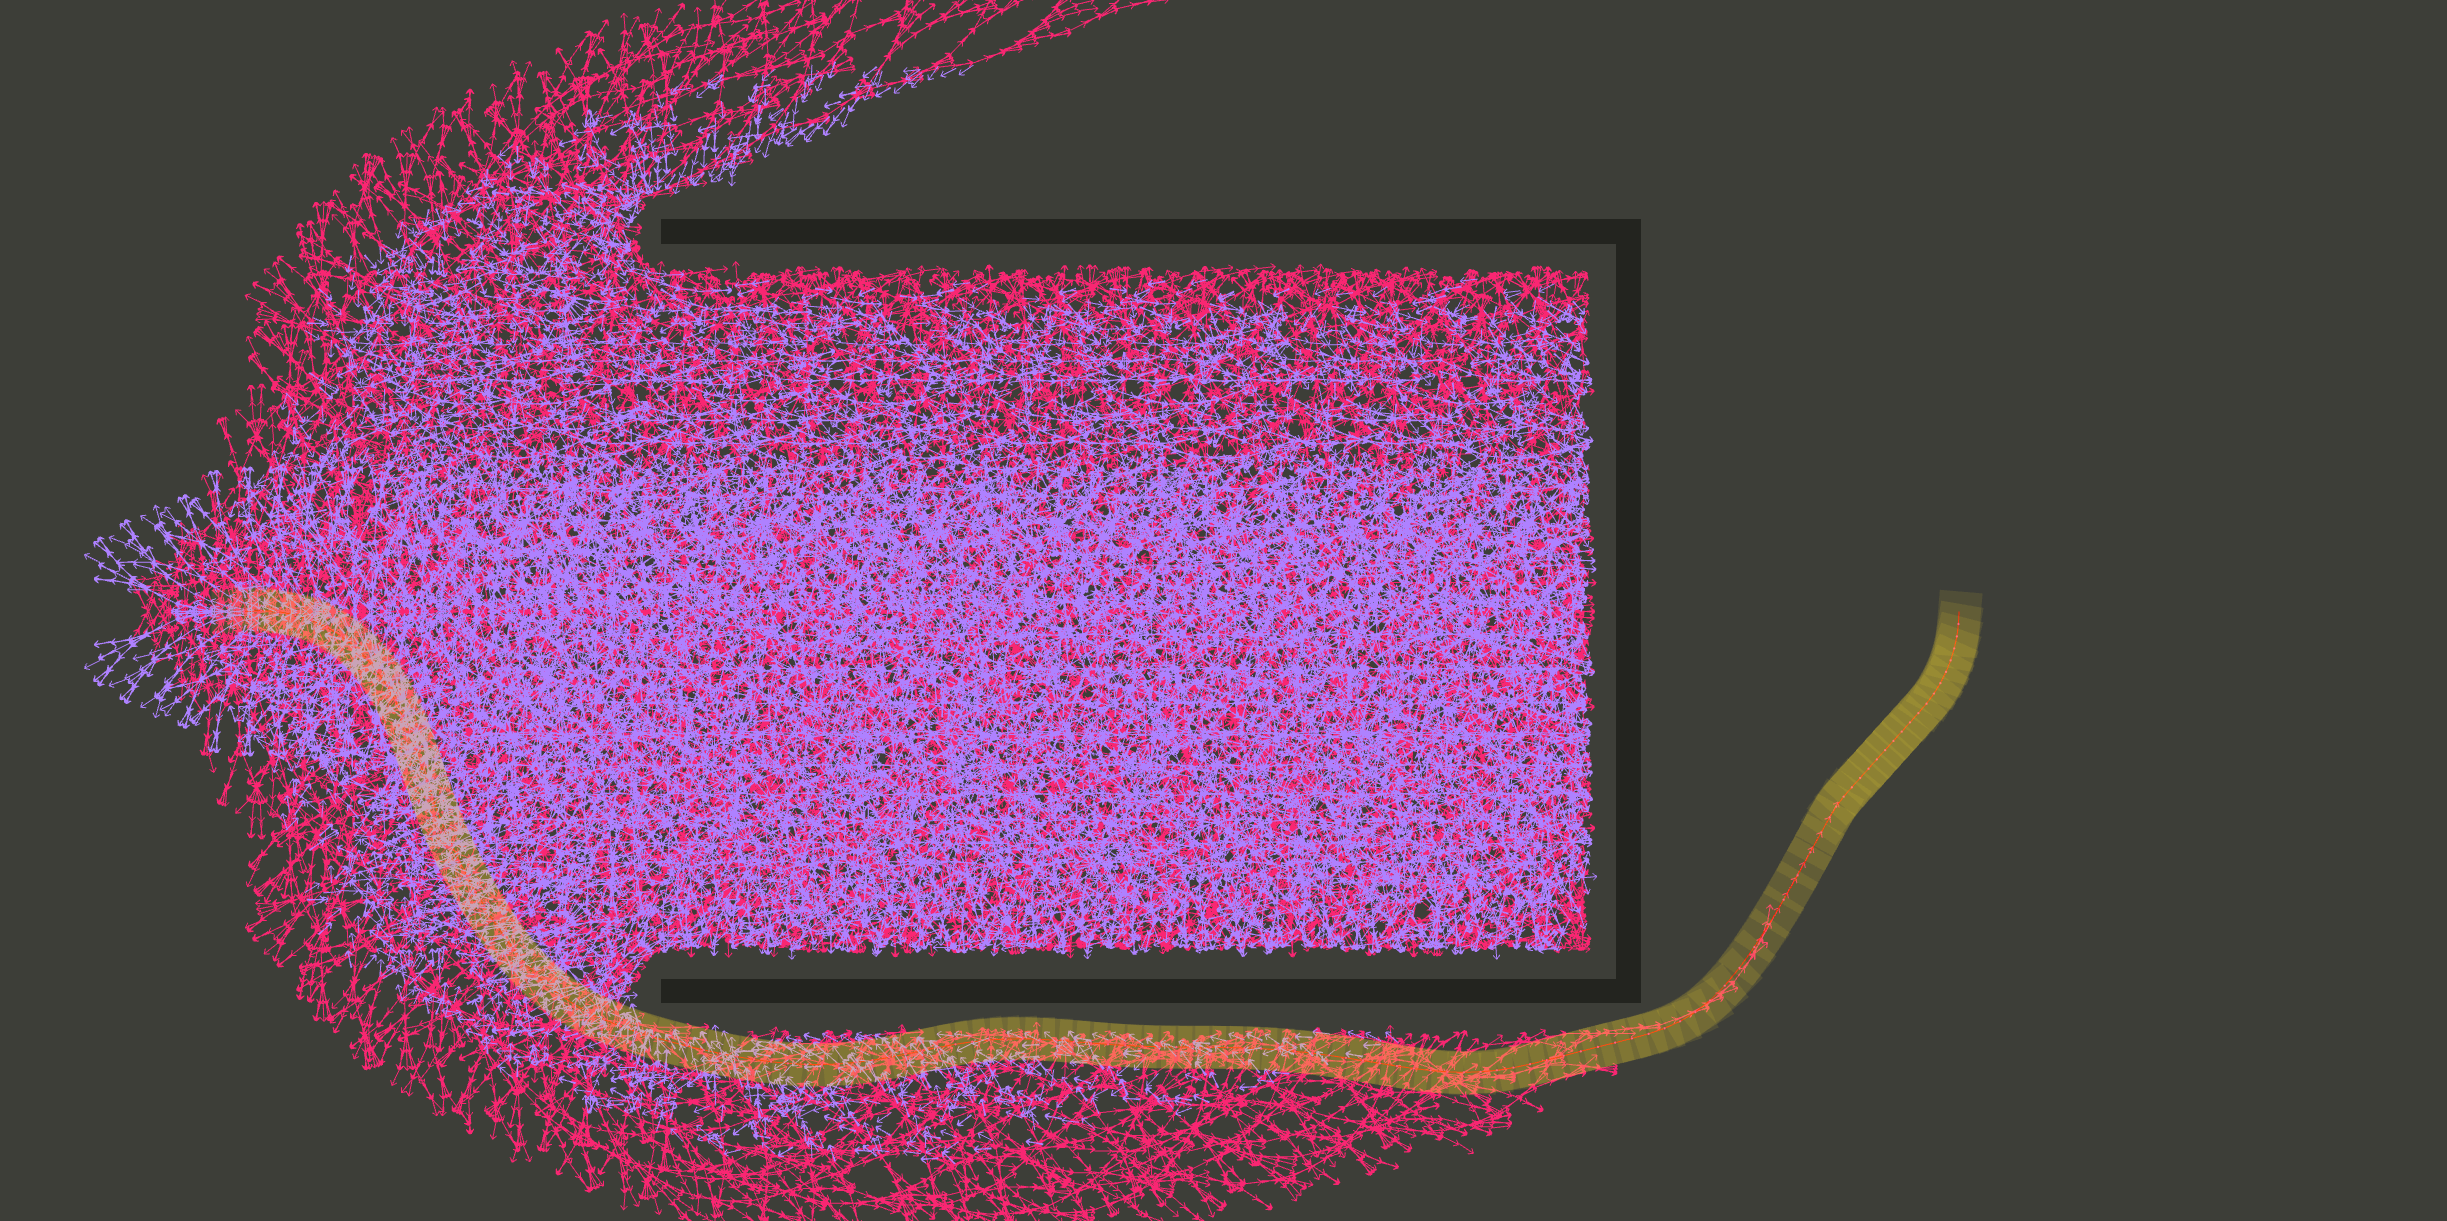
\includegraphics[width=\textwidth]{scenarioDeadEnd.png}
        \caption{Euclidean, 72014 vertices, length 90.0001\,m}
        \label{fig:scenarioDeadEnd}
    \end{subfigure}
    \begin{subfigure}[t]{\textwidth}
        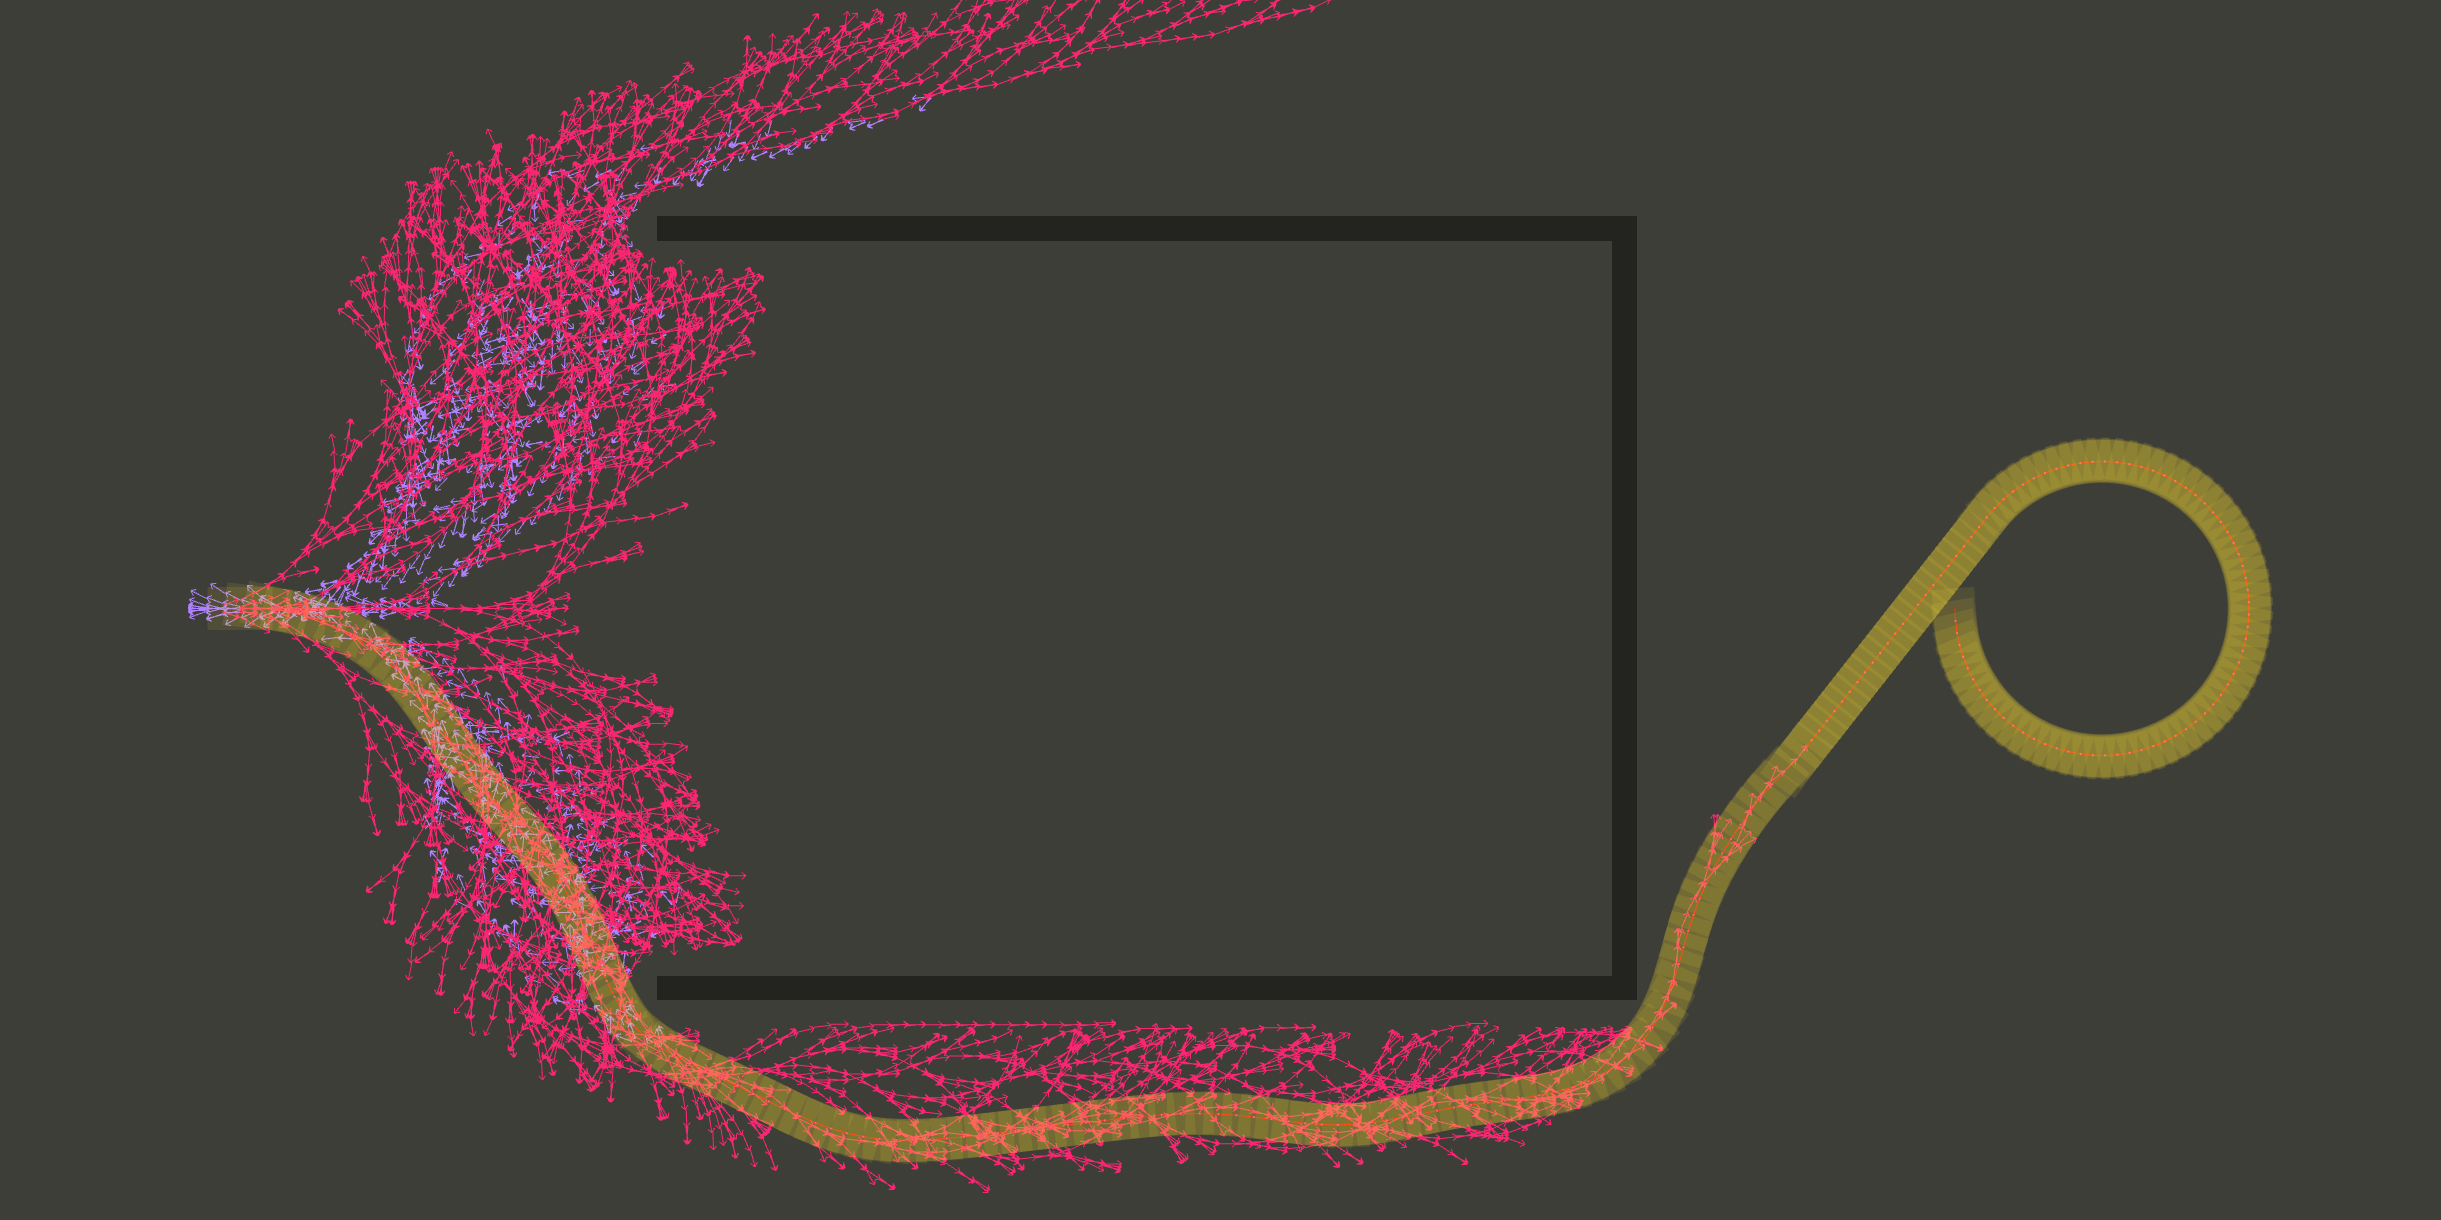
\includegraphics[width=\textwidth]{scenarioDeadEnd2d.png}
        \caption{2D A*, 8871 vertices, length 128.197\,m}
        \label{fig:scenarioDeadEnd2d}
    \end{subfigure}    
    \begin{subfigure}[t]{\textwidth}
        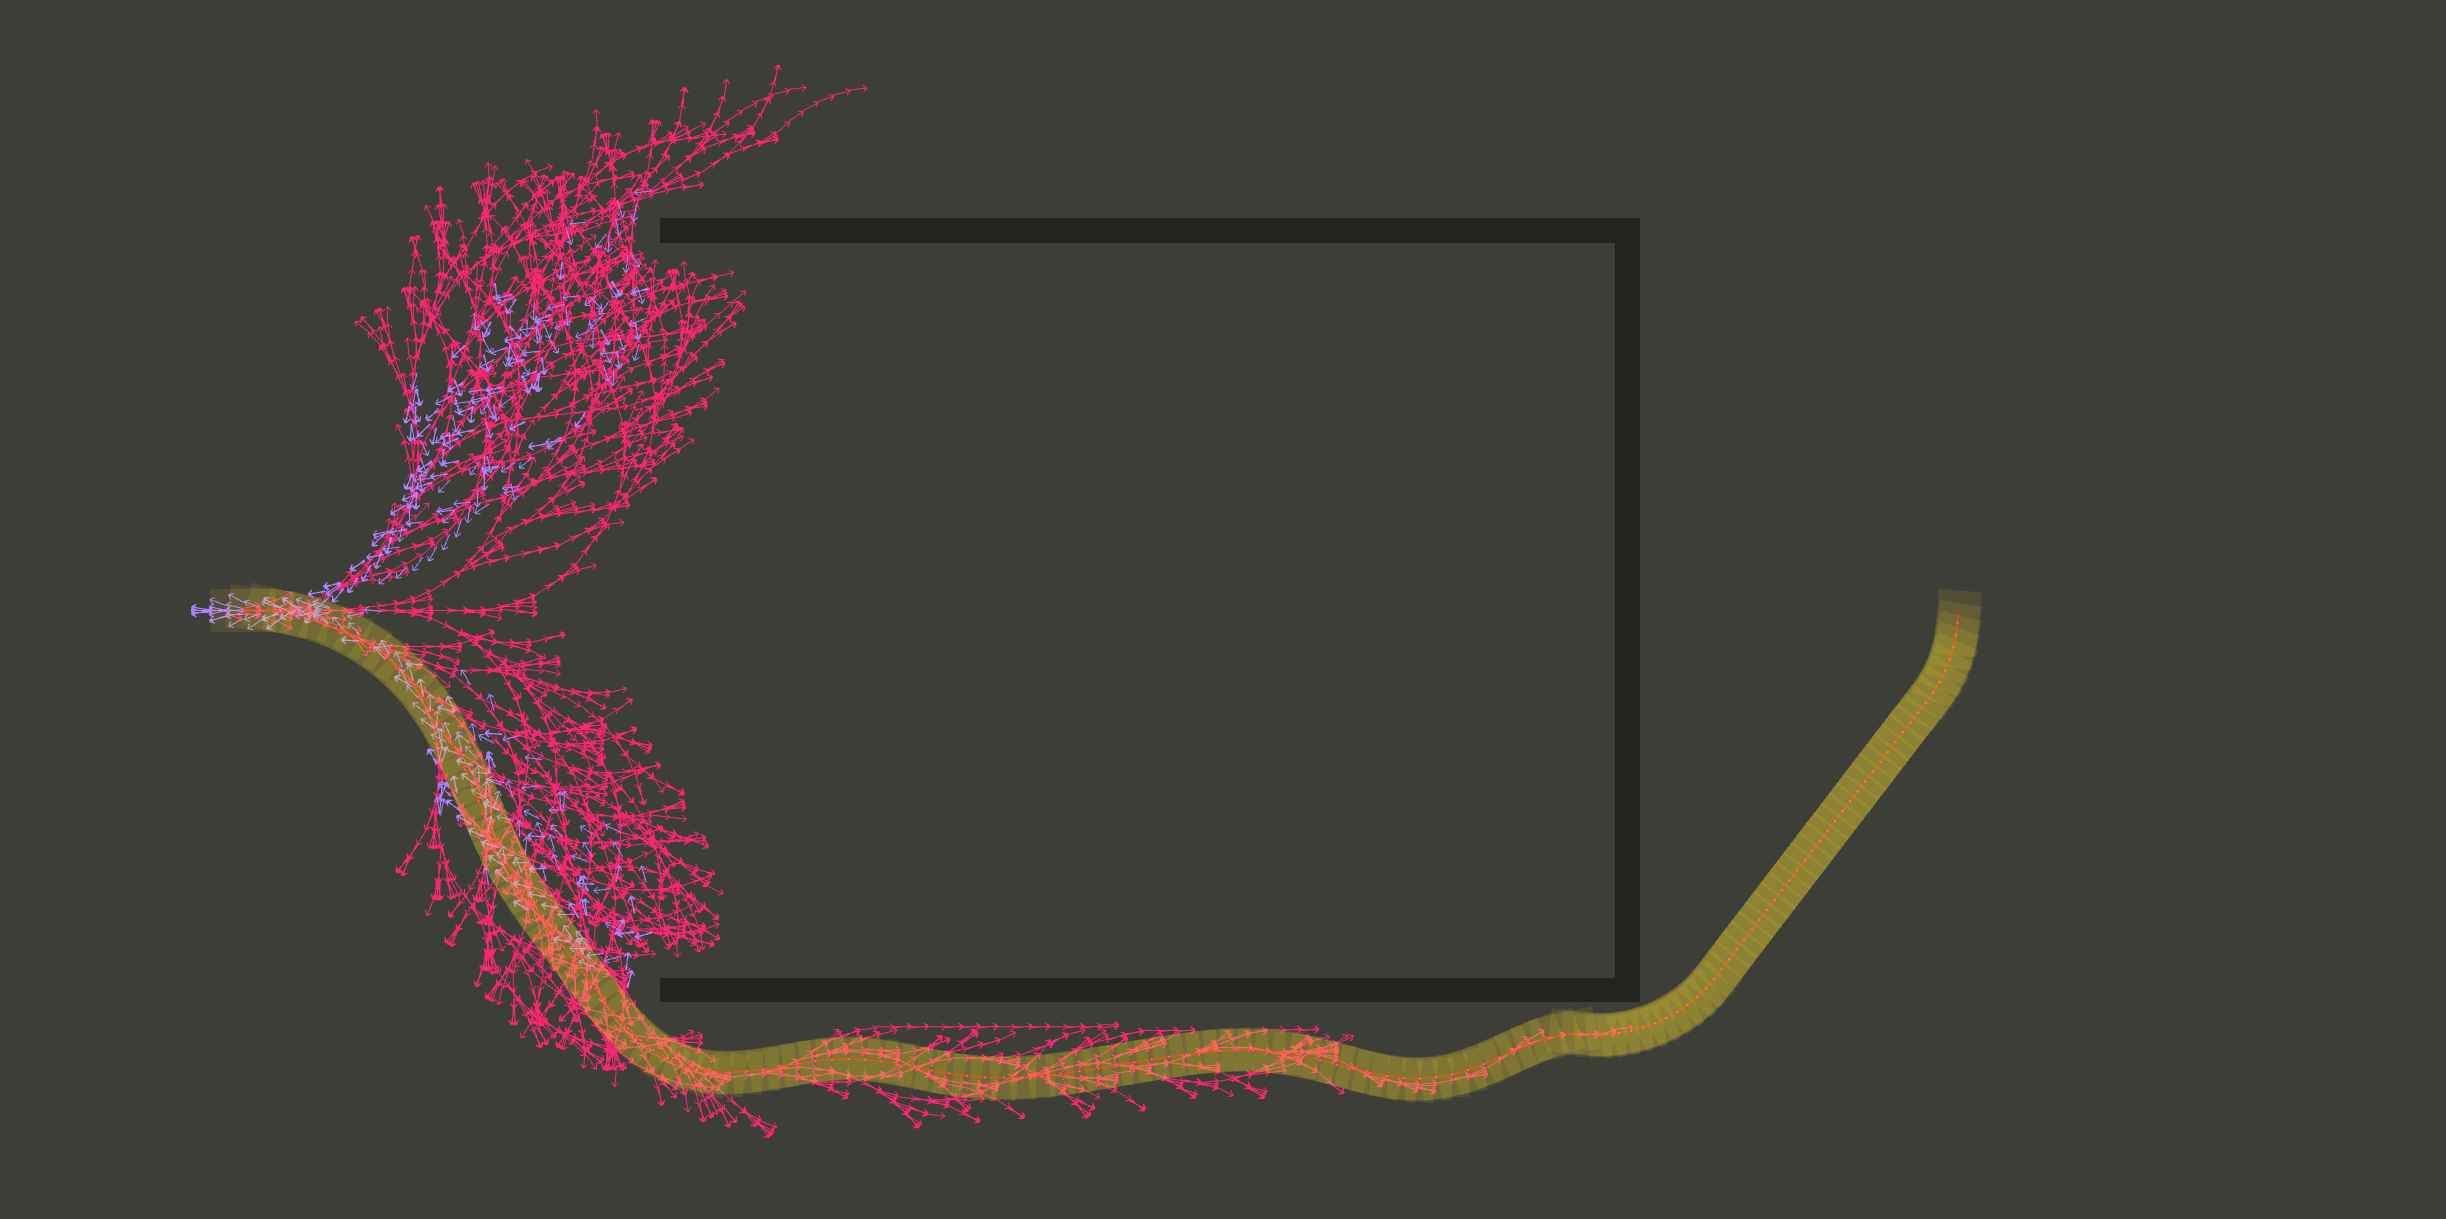
\includegraphics[width=\textwidth]{scenarioDeadEnd2dReedsShepp.png}
        \caption{2D A* \& Reeds Shepp, 8691 vertices, length 90.9778\,m}
        \label{fig:scenarioDeadEnd2dReedsShepp}
    \end{subfigure}
%    \begin{subfigure}[t]{\textwidth}
%        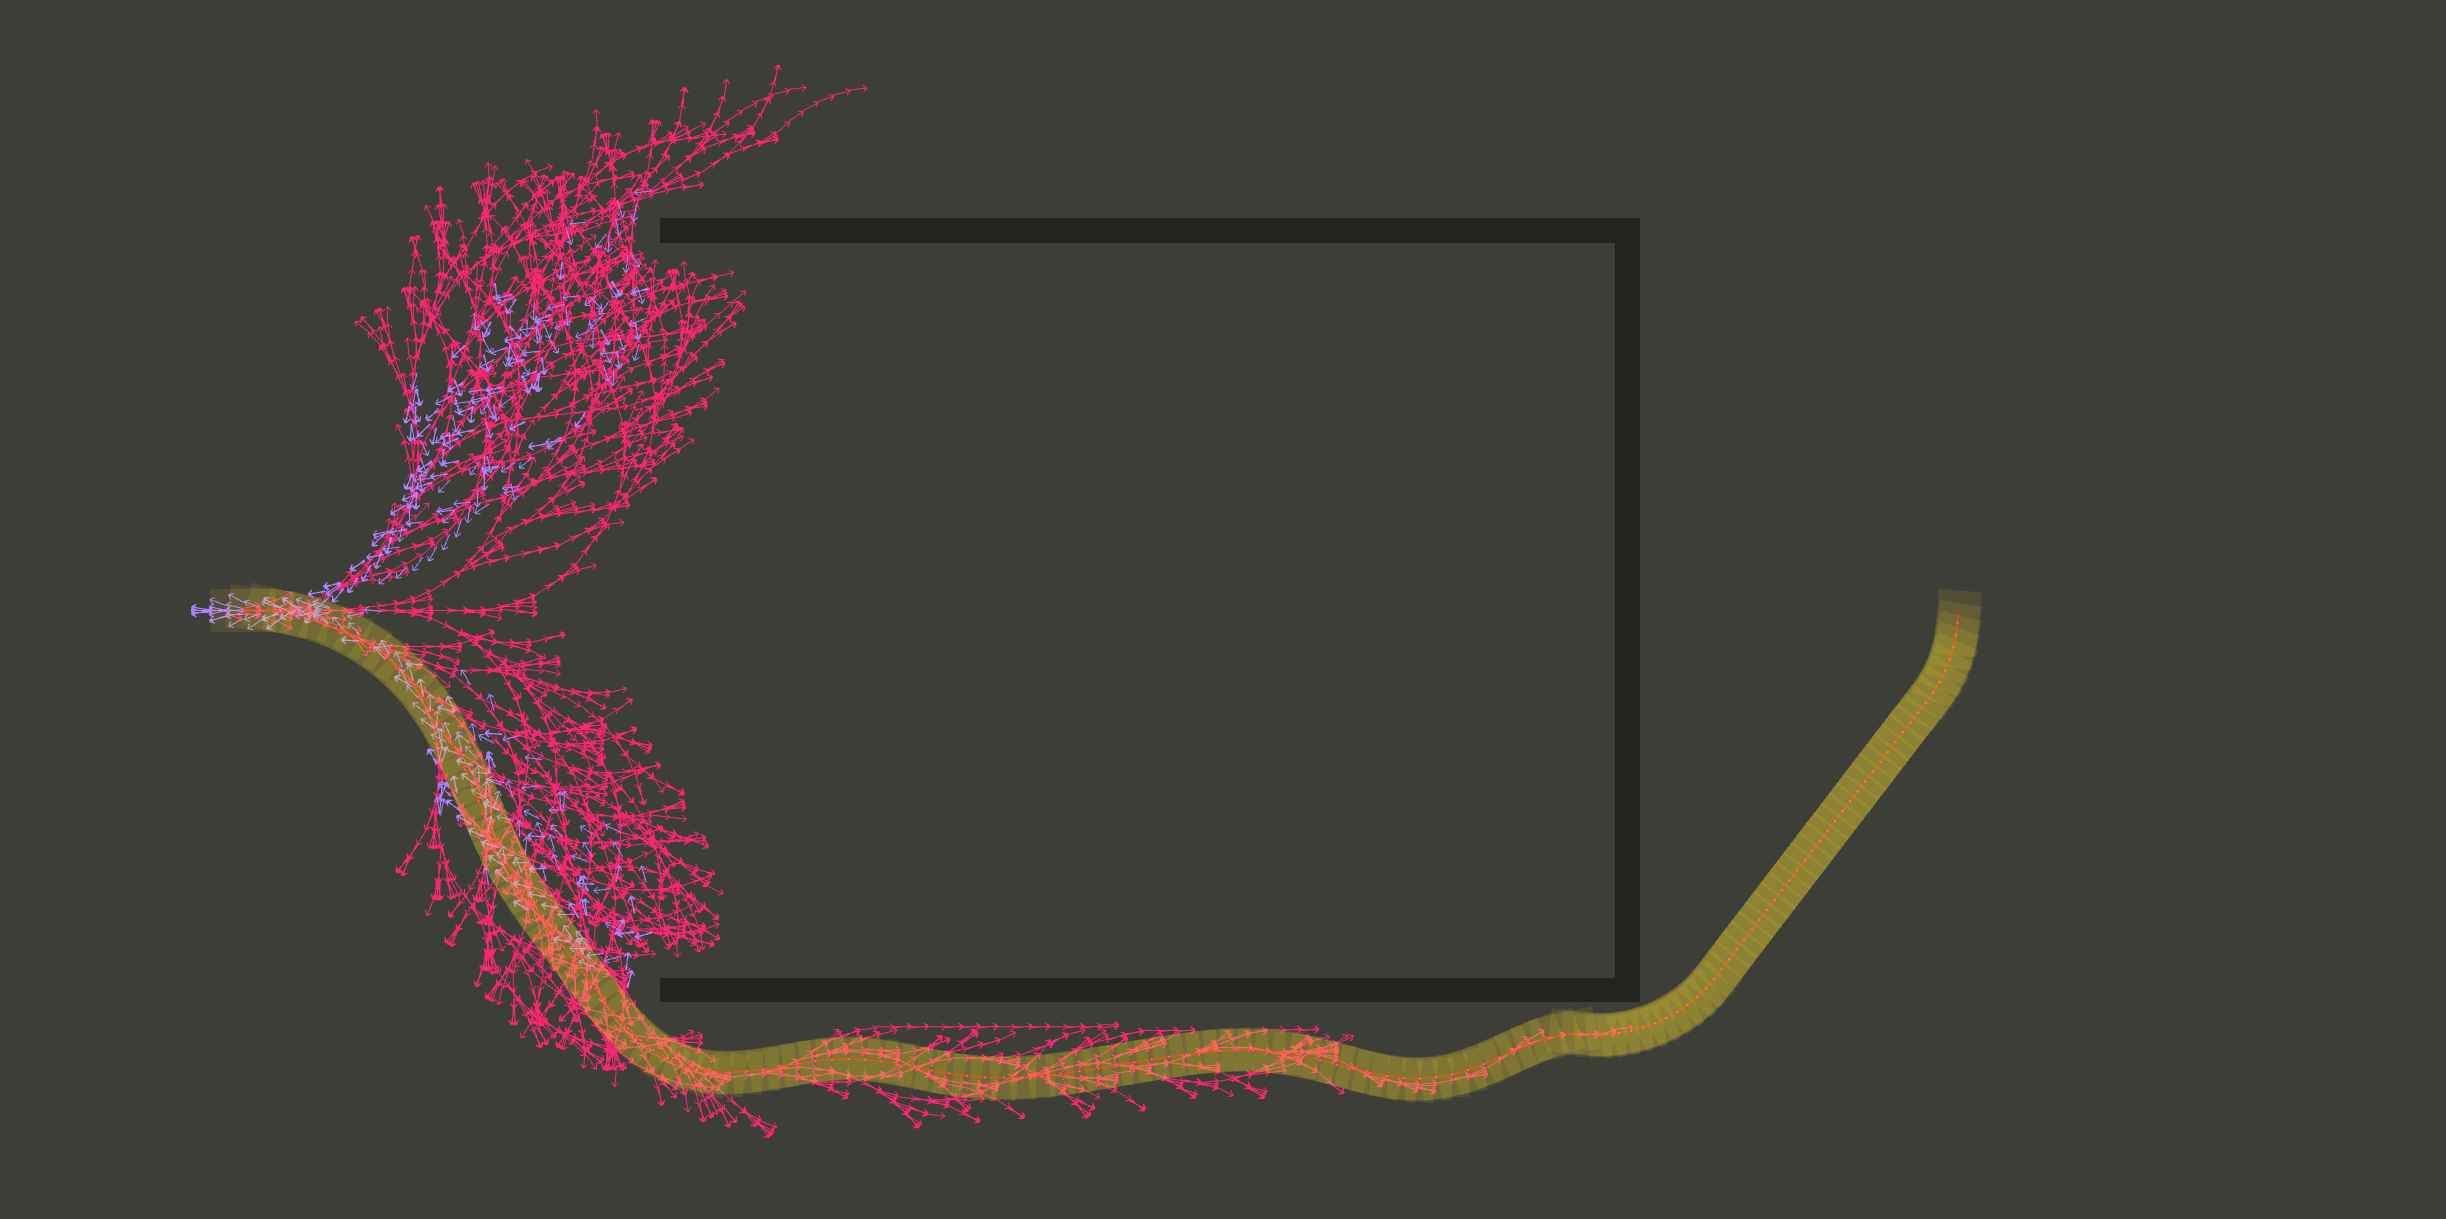
\includegraphics[width=\textwidth]{scenarioDeadEnd2dReedsShepp.png}
%        \caption{2D A* \& Dubins, 7829 vertices, length 91.5844\,m}
%        \label{fig:scenarioDeadEnd2dReedsShepp}
%    \end{subfigure}
    \caption{The dead end scenario}
    \label{fig:scenarioDeadEnd}
\end{figure}

\subsection{Additional Tests}

\begin{figure}[h]
    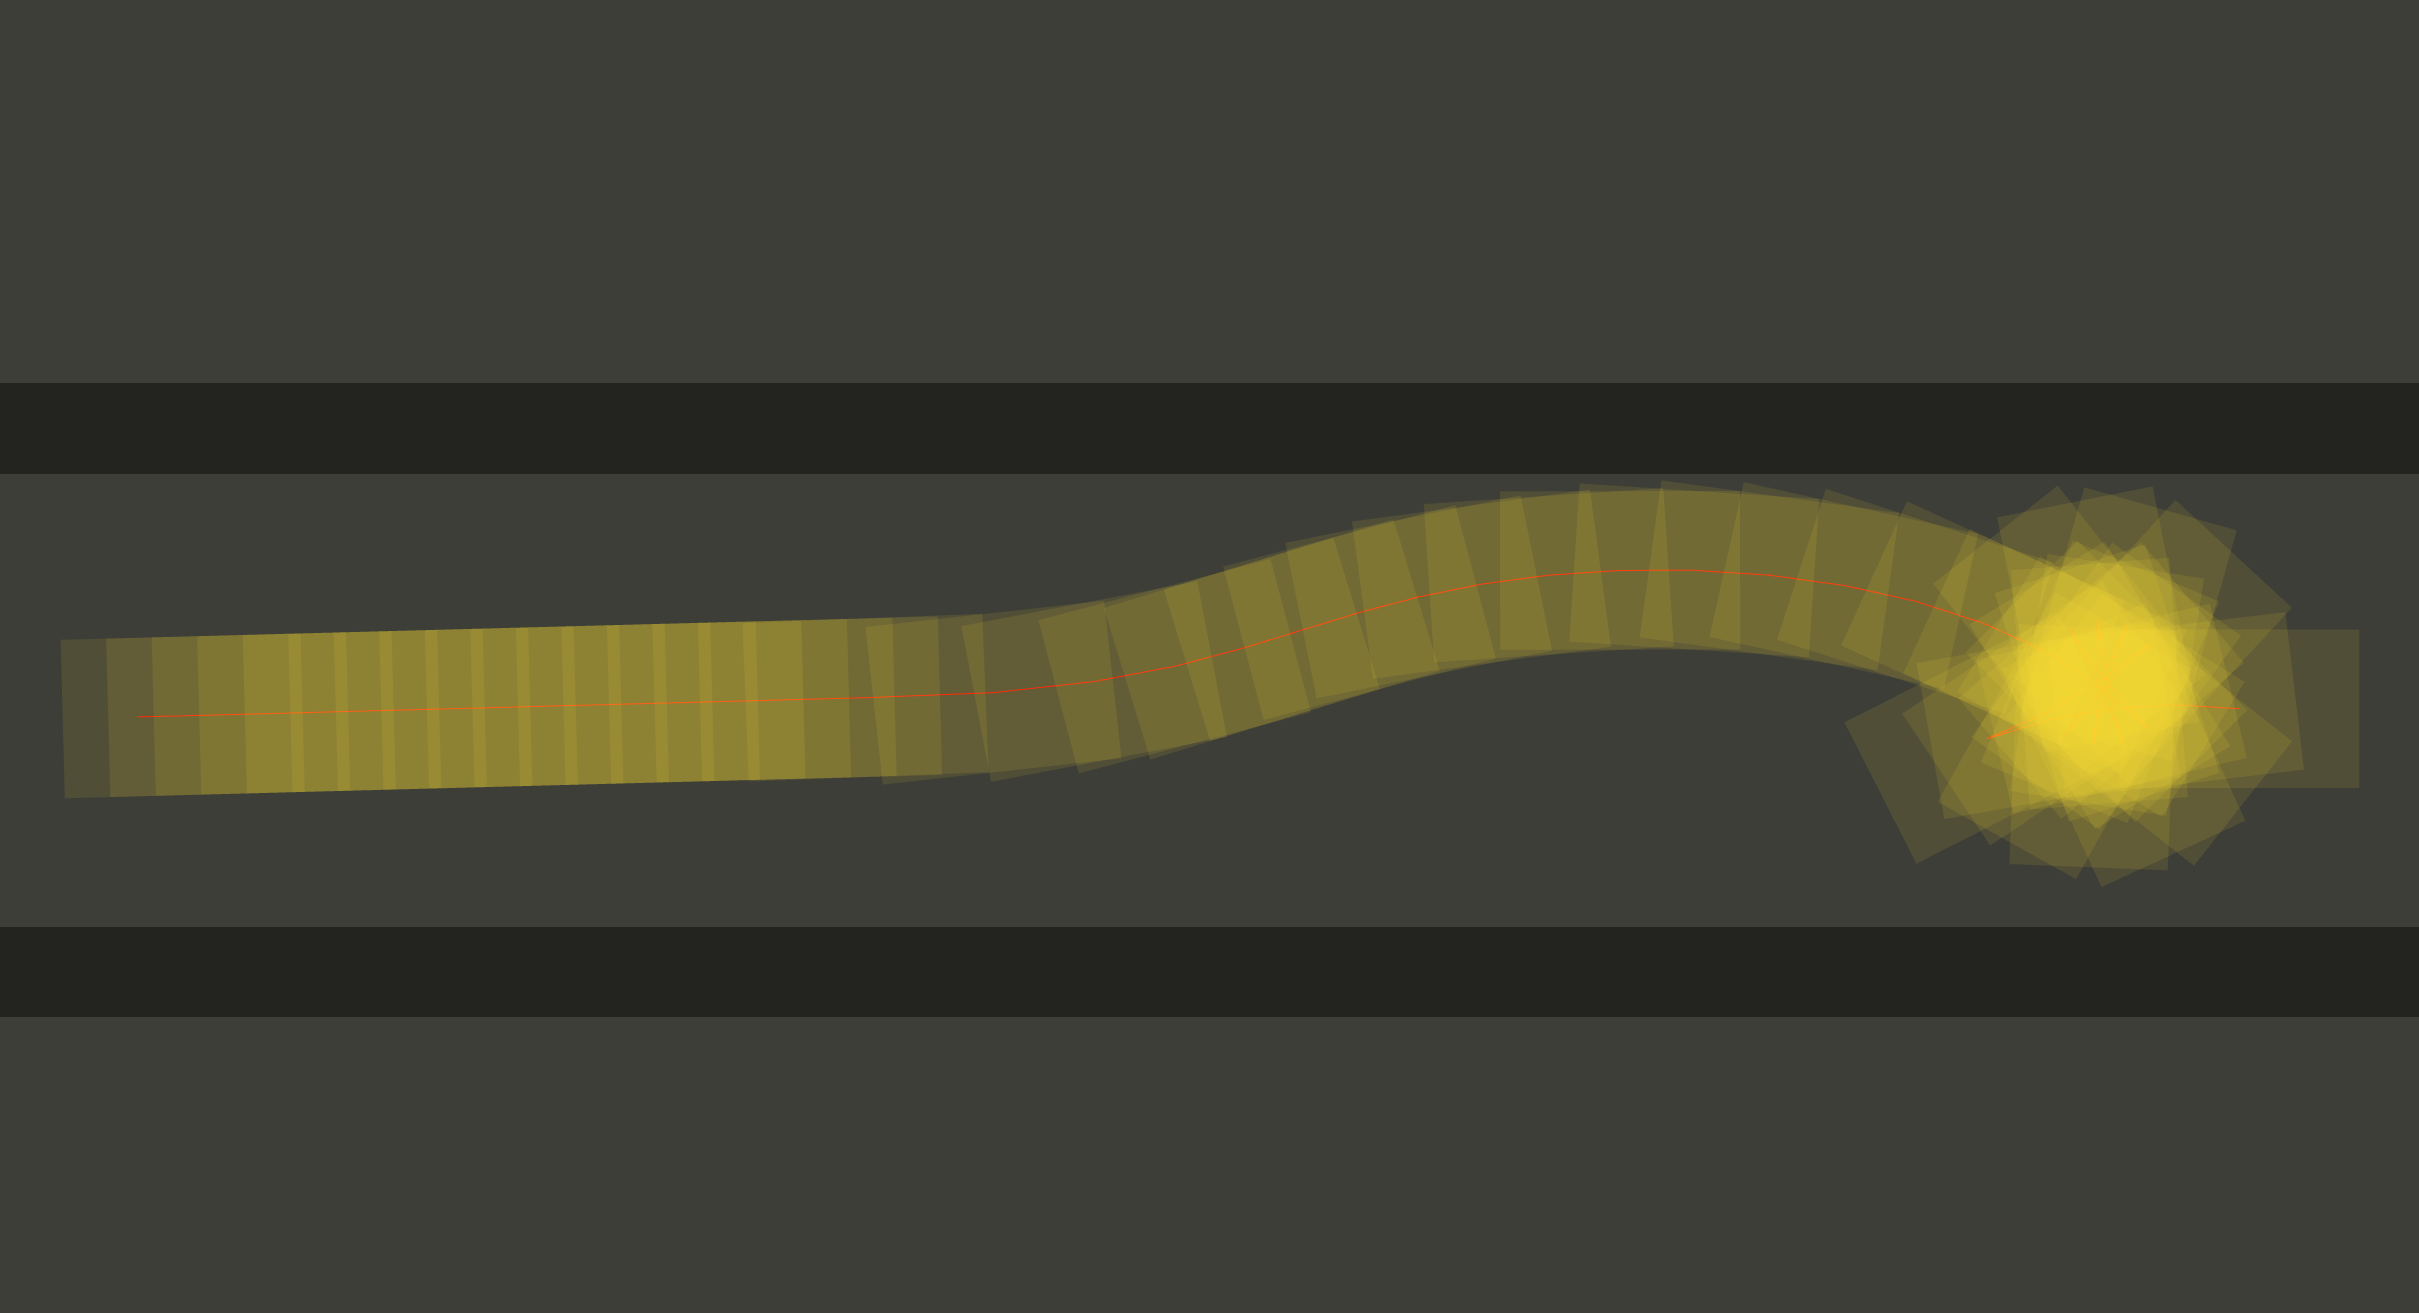
\includegraphics[width=\textwidth]{scenarioTurningSpot.png}
    \caption{Turning on the spot for change of directions}
    \label{fig:scenarioTurningSpot}
\end{figure}

\begin{figure}[h]
    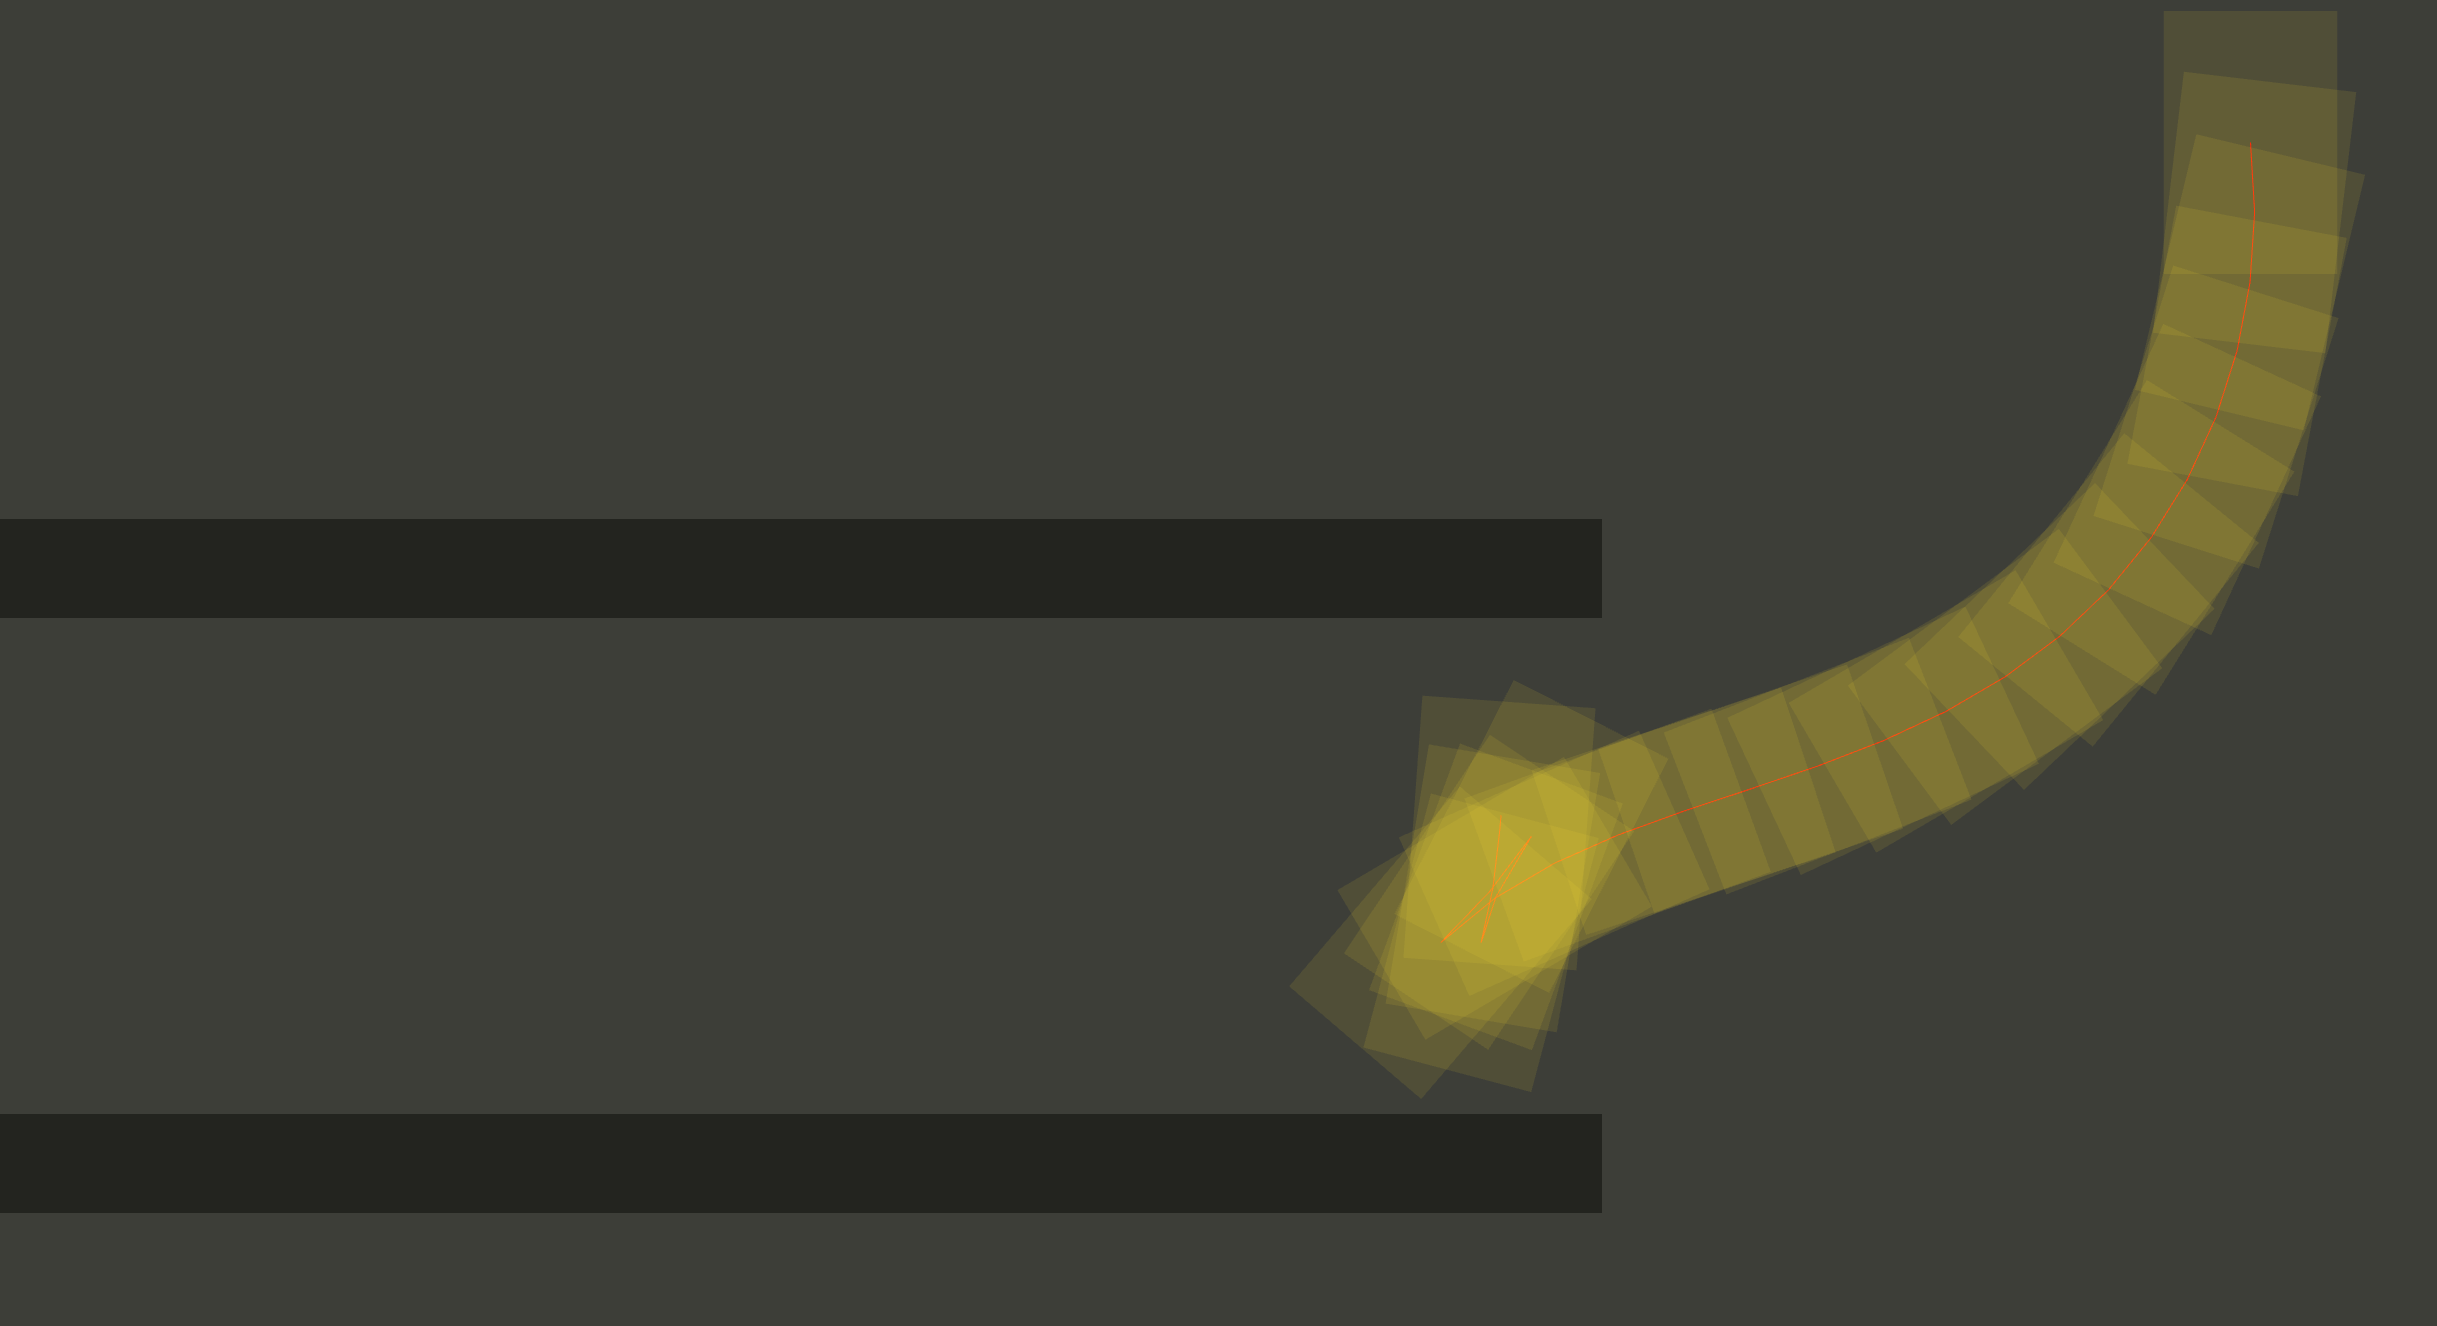
\includegraphics[width=\textwidth]{scenarioParallelParking.png}
    \caption{Parallel parking the car}
    \label{fig:scenarioParallelParking}
\end{figure}

%\begin{figure}[h]
%    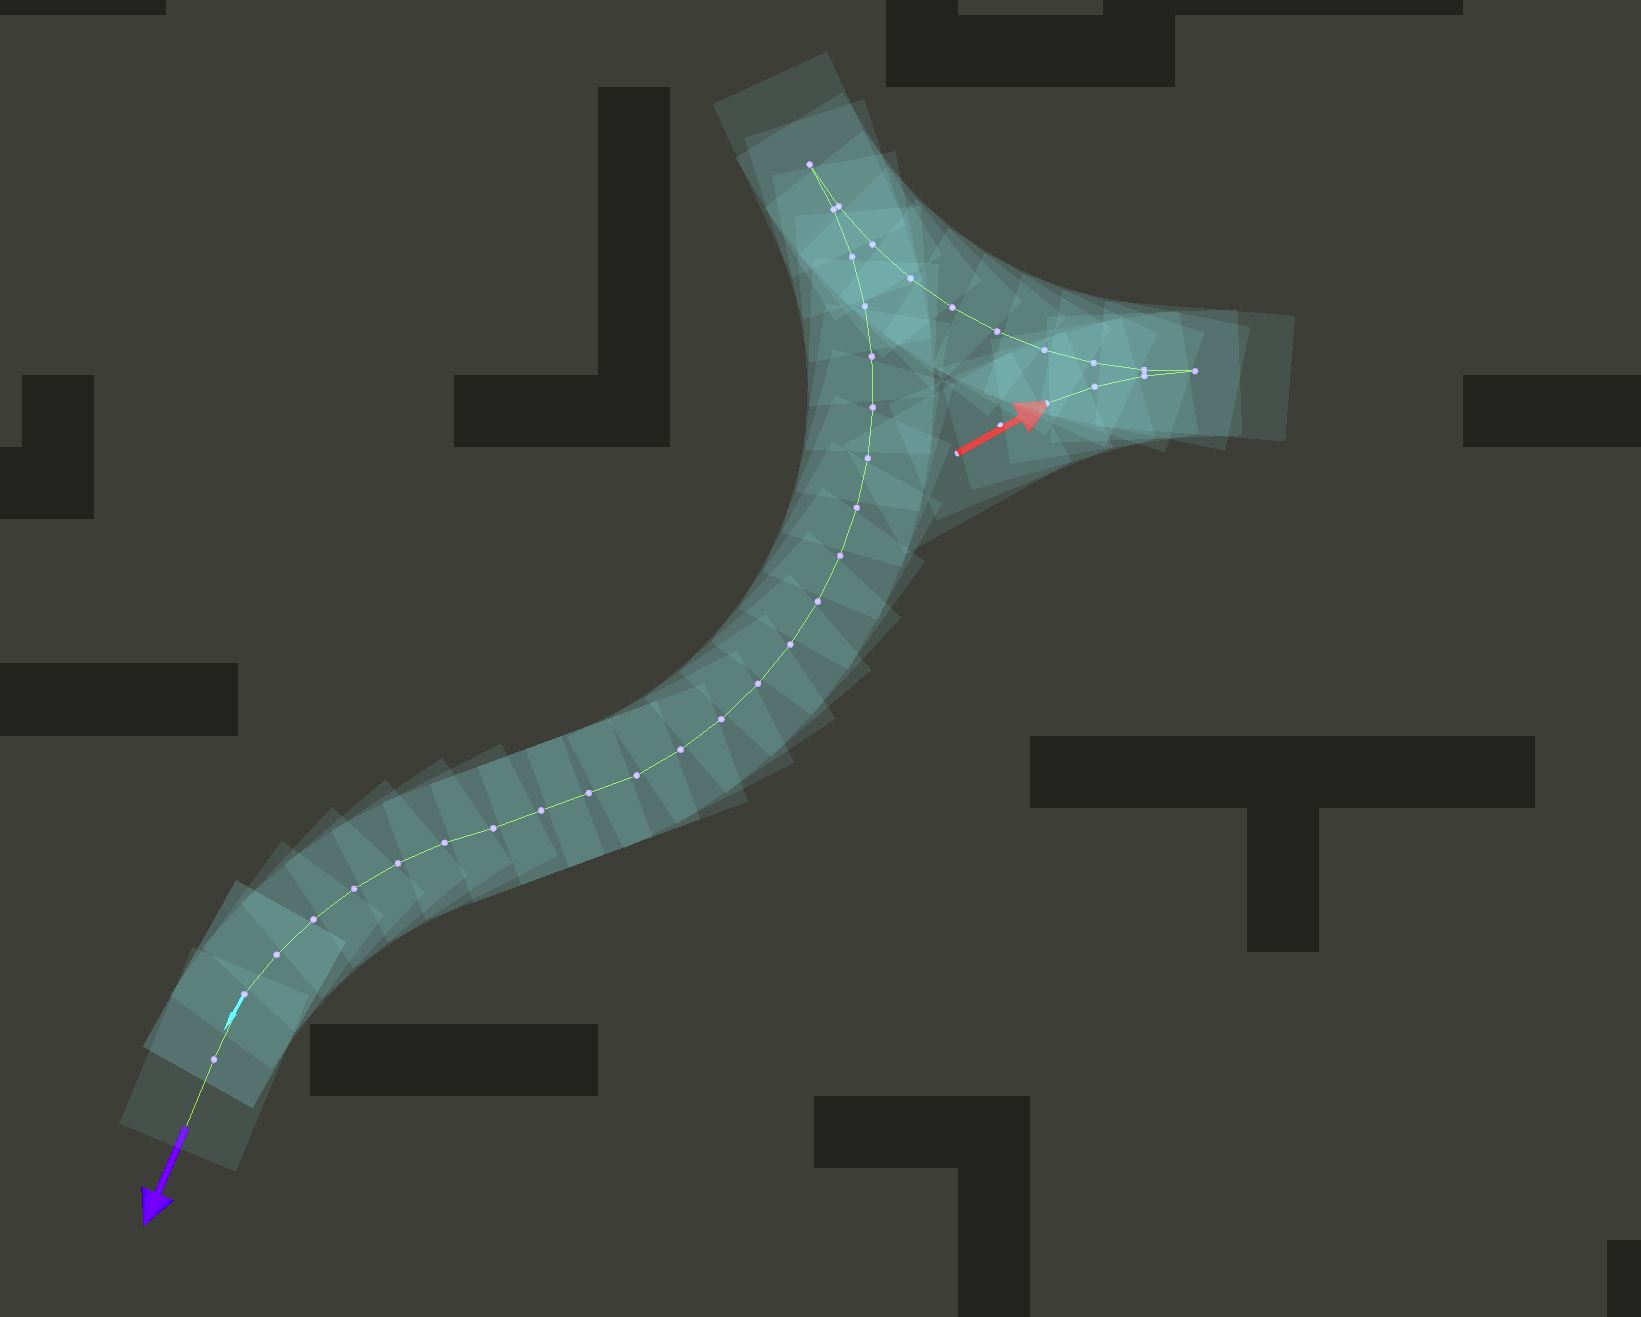
\includegraphics[width=\textwidth]{threePointTurn.png}
%    \caption{Three point turn for change of directions}
%    \label{fig:threePointTurn}
%\end{figure}
%
%\begin{figure}[h]
%    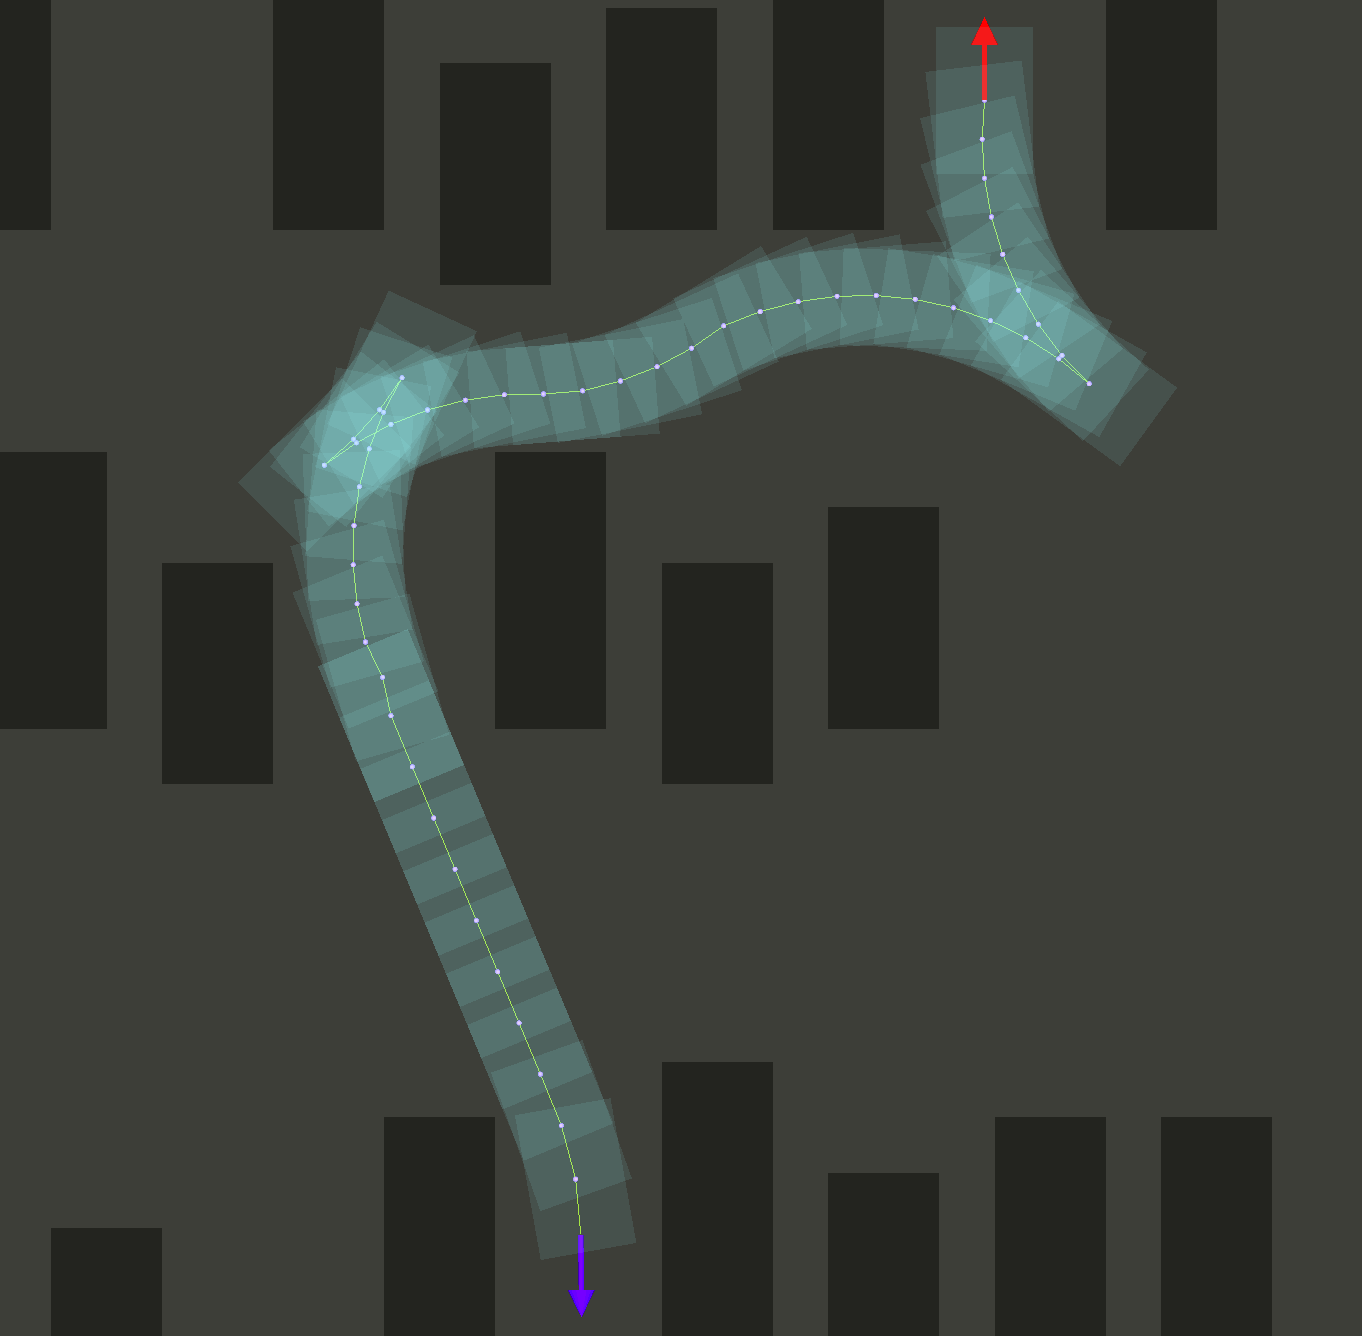
\includegraphics[width=\textwidth]{parking.png}
%    \caption{Change of parking spot in a parking lot}
%    \label{fig:parking}
%\end{figure}

\section{Real-world Results}